\documentclass{article}
\usepackage[polish]{babel}
\usepackage[a4paper,
    top=2cm,
    bottom=2cm,
    left=2cm,
    right=2cm,
    includehead]{geometry}
\usepackage{amsmath}
\usepackage{graphicx}
\usepackage[colorlinks=true, allcolors=black]{hyperref}
\usepackage{fancyhdr}
\usepackage[T1]{fontenc}
\usepackage{subcaption}
\usepackage{lastpage}
\usepackage{float}

\pagenumbering{arabic}
\pagestyle{fancy}
\fancyhf{}
\rhead{Dominik Adamczyk, Szymon Nowak-Trzos}
\lhead{Obliczanie grafu widoczności}
\fancyfoot[R]{Strona \thepage \hspace{1pt} z \pageref{LastPage}}
% \font\titleFont=ComicSansat 36pt
% \font\authorFont=cmr12 at 20pt


\title{\Huge Obliczanie grafu widoczności \\
\Huge Sprawozdanie \ \\ \ \\}
\author{\Large Dominik Adamczyk \\ \Large Szymon Nowak-Trzos \\ grupa nr 2 \\ Algorytmy geometryczne 2022/2023}
\date{}


\begin{document}
\maketitle

\newpage
\tableofcontents
\newpage

\section{Specyfikacja techniczna}
\qquad Projekt został stworzony w języku JavaScript przy użyciu biblioteki p5.js w wersji 1.5.0. Wszystkie testy przeprowadzono na komputerach, następującej specyfikacji technicznej, różniących się jedynie systemem operacyjnym:
\begin{itemize}
\item procesor: Intel Core i5-1135G7
\item pamięć ram: 16 GB
\item system operacyjny: Windows 10 Home x64 / Windows 11 Home x64.
\end{itemize}
\noindent \qquad Program napisany został w środowisku Visual Studio Code, a jego testy przeprowadzono poprzez uruchomienie go na lokalnym i zewnętrznym serwerze przy pomocy przeglądarek Google Chrome i Brave.


\section{Wstęp teoretyczny i opis problemu}
\subsection{Cel zadania}
\qquad Celem ćwiczenia było zaimplementowanie algorytmu pozwalającego znajdować graf widoczności dla zbioru rozłącznych wielokątów zadanych przez użytkownika, a także stworzenie wizualizacji pozwalających przedstawić działanie implementowanego algorytmu, z uwzględnieniem poszczególnych kroków.
\subsection{Opis zagadnienia}

\qquad Graf widoczności to graf, który dla zadanego zbioru rozłącznych wielokątów określa wszystkie połączenia między ``widzącymi się'' wierzchołkami. Są to takie wierzchołki, pomiędzy którymi można przeprowadzić odcinek taki, że ten nie będzie przecinał żadnej krawędzi wielokąta. Na potrzeby tego zadania przyjmujemy, że zadany zbiór wielokątów jest zbiorem otwartym (wierzchołki ani krawędzie tworzące wielokąty nie należą do nich), czyli punkty będące sąsiadującymi wierzchołkami wielokąta ``widzą się'' wzajemnie (ponieważ krawędź nie jest elementem wielokąta). Takie podejście skutkuje tym, że w wynikowym grafie widoczności zawarte zostają wszystkie krawędzie należące do zbioru wielokątów wejściowych. Rozwiązanie to, chociaż przydatne w kontekście zastosowań algorytmu, niesie za sobą pewne konsekwencje implementacyjne, które będą opisywane w dalszej części sprawozdania.

\noindent \qquad Naiwny algorytm rozwiązujący powyższy problem nie jest skomplikowany - do jego wykonania wystarczy dla każdej pary wierzchołków sprawdzić, czy istnieje krawędź przecinająca odcinek tworzony przez te wierzchołki. Przedstawiony algorytm ma mało zadowalającą złożoność - $O(n^3)$, gdzie n to liczba krawędzi zbioru wejściowego - takie oznaczenie przyjęte jest w całym sprawozdaniu. Implementowany w tym projekcie algorytm osiąga złożoność $O(n^2*log(n))$.

\begin{figure}[ht]
\caption{}
\centering
\begin{subfigure}{.5\textwidth}
\centering
\caption{Przykładowy zestaw danych wejściowych}
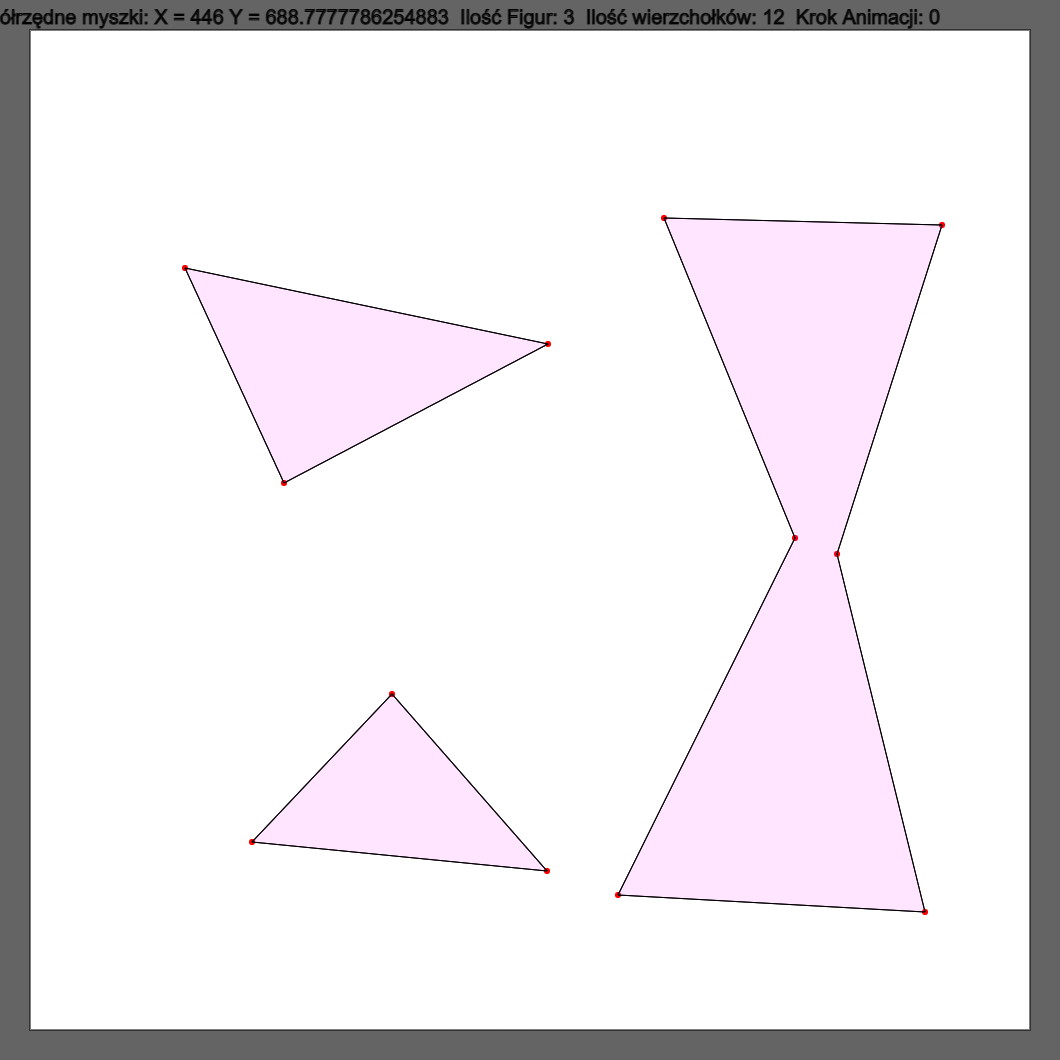
\includegraphics[width=.75\linewidth]{rys1a.png}
\end{subfigure}%
\begin{subfigure}{.5\textwidth}
\centering
\caption{Graf widoczności dla przykładowego zbioru}
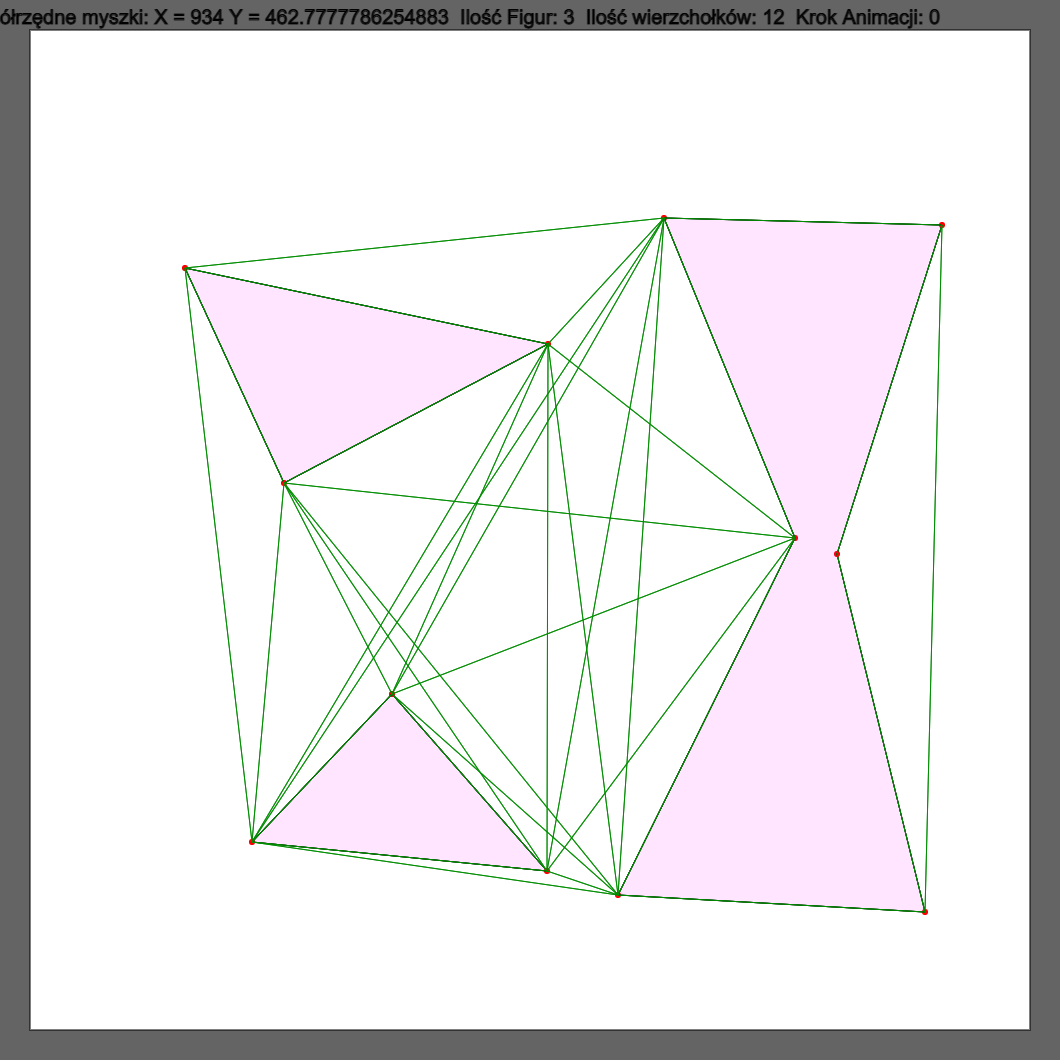
\includegraphics[width=.75\linewidth]{rys1b.png}
\end{subfigure}%
\end{figure}


\section{Opis algorytmu}
\subsection{Główny algorytm}
\qquad Główna część algorytmu nie jest skomplikowana (na potrzeby sprawozdania nazwiemy ją \textbf{grafWidoczności}). Idea wyznaczenia grafu widoczności polega na wyznaczeniu wszystkich widocznych wierzchołków dla każdego z wierzchołków należących do danych wejściowych. Algorytm wyznaczenia widocznych wierzchołków (\textbf{widoczneWierzchołki}) będzie w takim razie wykonywany $O(n)$ razy - liczba wierzchołków w zbiorze wejściowym jest powiązana z jego liczbą krawędzi i wielokątów. 
\subsection{Algorytm \textbf{widoczneWierzchołki}}
\qquad W celu uzyskania złożoności $O(n^2*log(n))$ konieczne jest aby wyznaczanie wszystkich punktów widocznych z zadanego wierzchołka $P$ odbywało się w czasie $O(n*log(n))$. Aby uzyskać taki efekt wykorzystywany jest algorytm czerpiący koncepcję z algorytmów zamiatania. Różnice względem typowych algorytmów zamiatania (np. algorytmu wyznaczającego przecięcia odcinków) są w tym przypadku takie, że struktura zdarzeń nie zmienia się w trakcie pracy algorytmu, a struktura stanu (miotła) nie przesuwa się wzdłuż pewnej osi, a obraca dookoła punktu $P$.

\noindent \qquad Pierwszym etapem wykonania tego algorytmu jest posortowanie wszystkich wierzchołków po ich rosnącym kącie pomiędzy pewnym ustalonym wektorem, a wektorem wodzącym pomiędzy punktem $P$, a rozważanym wierzchołkiem (przeciwnie do ruchu wskazówek zegara). Dla tych samych kątów sortowanie odbywa się rosnąco na podstawie odległości pomiędzy punktem $P$, a wierzchołkiem. Tak posortowane punkty tworzą strukturę zdarzeń.

\noindent \qquad  Strukturą stanu jest zrównoważone drzewo poszukiwań binarnych, na którym będą przechowywane krawędzie aktualnie przecinające się z miotłą. Miotłę należy interpretować jako półprostą wychodzącą z punktu $P$ i przechodzącą przez kolejne punkty ze struktury zdarzeń - na samym początku algorytmu miotła przechodzi przez pierwszy punkt struktury zdarzeń. Po zainicjowaniu na strukturze stanu umieszczane są wszystkie krawędzie wielokątów, które przecinają miotłę w jej początkowej pozycji. Porządek krawędzi umieszczanych na drzewie jest zadany poprzez rosnącą odległość między punktem $P$, a przecięciem odcinka z miotłą. Warto zwrócić uwagę, że względny porządek pomiędzy krawędziami na miotle nie ulega zmianie - krawędzie wielokątów nie mogą się przecinać.

\noindent \qquad Przy pomocy tak zainicjowanych struktur danych możliwy jest do wykonania właściwy algorytm. Polega on na iteracji po każdym z punktów w strukturze zdarzeń i wykonaniu na nim odpowiednich akcji. Pierwszą z akcji jest sprawdzenie, czy wierzchołek na którym jesteśmy jest widoczny (odpowiada za to osobna funkcja \textbf{czyWidoczny}), a jeżeli tak, to ta informacja jest zapisywana. Następnie należy określić dwie krawędzie wychodzące z aktywnego wierzchołka. Jeżeli któraś z tych krawędzi (albo obydwie) jest po prawej stronie miotły, to nie będzie więcej tworzyła z nią przecięcia (miotła obraca się w kierunku przeciwnym do ruchu wskazówek zegara), więc krawędź ta jest zdejmowana ze struktury stanu, na której musiała dotychczas być. Jeżeli natomiast krawędzie znajdują się po lewej stronie miotły, to są dodawane do struktury stanu. Przedstawione w tym kroku operacje (włącznie z funkcją \textbf{czyWidoczny}) mają złożoność $O(log(n)$ (są to operacje na zrównoważonym drzewie) i powtórzone są $O(n)$ razy, co sprawia, że ten etap ma złożoność $O(n*log(n))$ - taką samą jak sortowanie, które przeprowadzane jest na początku opisywanej funkcji.

\begin{figure}[ht]
\centering
\caption{Przykładowy wynik działania \textbf{widoczneWierzhołki}}
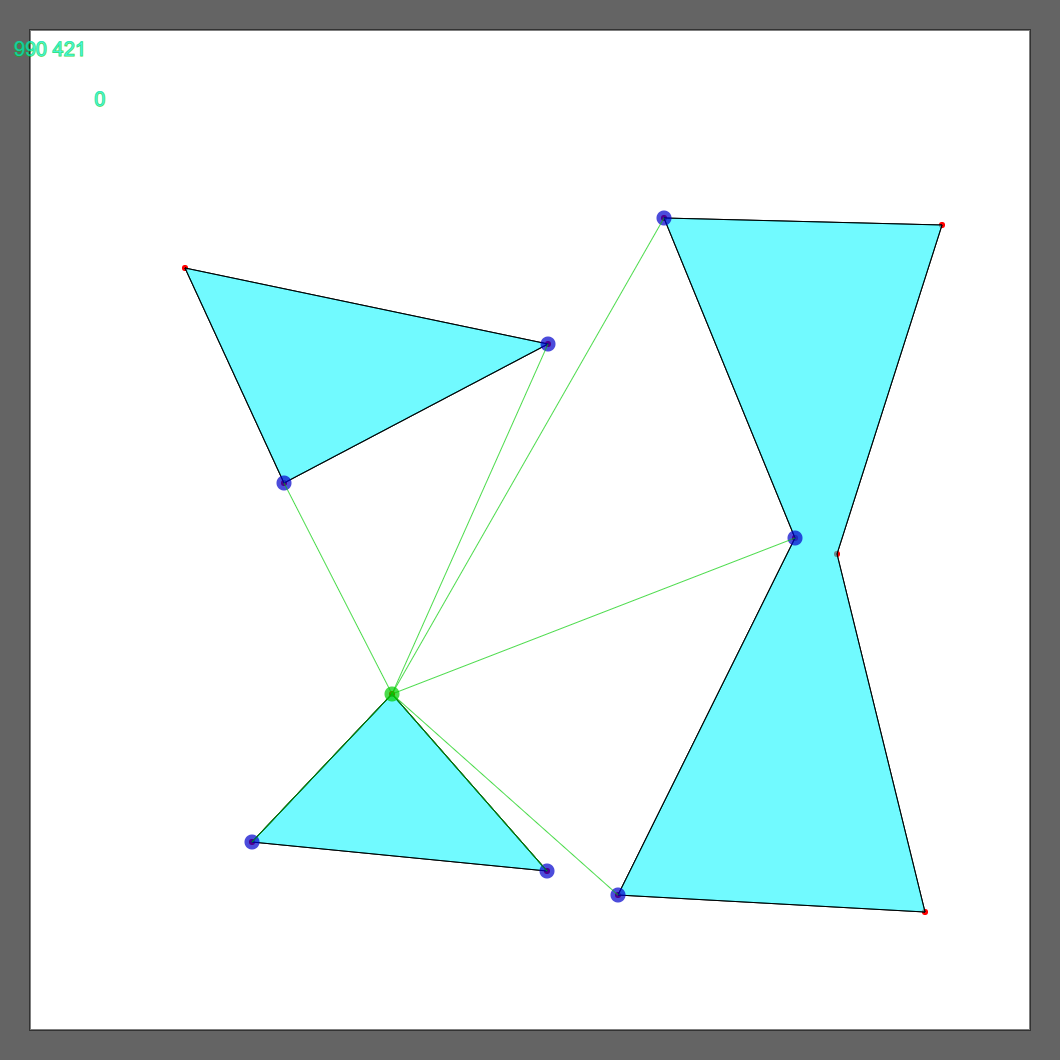
\includegraphics[width=0.5\linewidth]{rys2.png}
\end{figure} 

\subsection{Algorytm \textbf{czyWidoczny}}

\noindent \qquad Na tym etapie konieczne jest sprawdzenie, czy odcinek $\overline{Pw_i}$ tworzony przez dwa zadane wierzchołki - $P$, $w_i$ -  jest przecinany przez jakikolwiek odcinek w drzewie. W tym celu należy rozważyć parę przypadków. Pierwszym z nich jest sprawdzenie czy $\overline{Pw_i}$ przechodzi przez środek wielokąta przy wierzchołku $w_i$ - jeżeli tak, to zwracany jest fałsz. Kolejno sprawdzany jest przypadek gdy $w_i$ jest albo pierwszym wierzchołkiem, albo $P$, $w_i$, $w_{i-1}$ nie są współliniowe. Wtedy wystarczy sprawdzić wysunięty najbardziej na lewo liść w drzewie opisanym w poprzednim punkcie. Jeżeli krawędź przechowywana w tym liściu przecina $\overline{Pw_i}$, to zwracany jest fałsz, a w przeciwnym wypadku prawda. Jeżeli jednak w poprzednim warunku okazało się, że $P$, $w_i$, $w_{i-1}$ są współliniowe należy oprzeć następne kroki o status wierzchołka $w_{i-1}$. Jeżeli nie był on widoczny, to $w_{i}$ też taki nie może być - wynika to z posortowania wierzchołków współliniowych. Jeżeli natomiast $w_{i-1}$ był widoczny, to należy przejść po całym drzewie i stwierdzić, czy istnieje krawędź przecinająca $\overline{w_{i-1}w_i}$. Jeżeli taka istnieje, to należy zwrócić fałsz, w przeciwnym wypadku - prawdę. Operacje w tej funkcji wykonywane są na zrównoważonym drzewie, co pozwala jej na uzyskanie złożoności $O(log(n))$. Przypadek widocznego współliniowego punktu $w_{i-1}$ można pominąć w obliczaniu złożoności, gdyż występuje rzadko.

\section{Szczegóły implementacji algorytmu}

\qquad Przedstawiony w poprzedniej sekcji algorytm pozostawia pewną dowolność podczas jego implementacji. Aby implementowany algorytm osiągał oczekiwaną złożoność obliczeniową, oraz działał poprawnie dla każdego zestawu danych wejściowych konieczne było rozwiązanie paru problemów.

\subsection{Reprezentacja punktu, odcinka i wielokąta}

\qquad Na potrzeby działania algorytmu zaimplementowane zostały odpowiednie klasy reprezentujące obiekty, na których przeprowadzane jest działanie algorytmu. Stworzone na te potrzeby klasy:

\begin{itemize}
\item Point - posiada współrzędne pojedynczego punktu
\item Line - Posiada dwa obiekty klasy Point wyznaczające odcinek
\item PointsCollection - przechowuje listę obiektów klasy Point
\item LinesCollection - przechowuje listę obiektów klasy Line
\item Shape - klasa reprezentująca wielokąt, przechowuje obiekt PointsCollection i LinesCollection. Kolejne punkty z PointsCollection wyznaczają wielokąt.
\item Scene - przechowuje wszystkie widoczne na ekranie
obiekty z klas wymienionych powyżej.
\end{itemize}

\noindent 
W powyższych klasach dodatkowo przechowywane są informacje konieczne do działania algorytmu, np. odnośniki danego punktu do krawędzi z niego wychodzących.

\noindent \qquad Jedną z istotnych informacji na temat obiektów klasy Shape jest sposób w jakim został zadany wielokąt (zgodnie, czy przeciwnie do ruchu wskazówek zegara). Jest to w szczególności przydatne do określania po której stronie trzech kolejnych punktów wielokąta jest jego środek (szczegóły użycia tej informacji przedstawione są w punkcie 4.5). W tym celu dla każdego wielokąta wyznaczany jest fragment jego otoczki wypukłej (pierwsze trzy kolejne punkty) przy pomocy algorytmu Jarvisa. Tak wyznaczone punkty stanowią zadany przeciwnie do ruchu wskazówek zegara fragment otoczki. Dzięki porównaniu ich kolejności z kolejnością punktów należących do wielokąta możliwe jest określenie orientacji w jakiej jest zadany.


\subsection{Znajdowanie punktu przecięcia odcinków}

\qquad Szukanie punktu przecięcia jest najczęściej powtarzaną operacją w algorytmie. W przypadku tej implementacji szukanie przecięcia odbywa się poprzez wyznaczenie równań prostych zawierających rozważane odcinki, a następnie rozwiązania odpowiedniego układu równań. Następnie sprawdzane jest, czy znaleziony punkt zawiera się w przedziałach wyznaczanych prostymi. Dodatkowo osobno rozważane są przypadki, gdy jedna z prostych jest pionowa - w ten sposób możliwe jest uniknięcie błędów z dzieleniem przez 0.

\subsection{Sortowanie punktów}

\qquad Algorytm \textbf{widoczneWierzchołki} w swoim pierwszym kroku wymaga posortowania punktów na podstawie ich kąta względem pewnego punktu początkowego $P$. Aby to zrobić korzystamy z algorytmu szybkiego sortowania, w którym funkcja komparatora polega na użyciu wyznacznika o wzorze 
$det(a, b, c) = \begin{vmatrix}
a_x - c_x && a_y - c_y \\ b_x - c_x && b_y - c_y.
\end{vmatrix}$.
W ten sposób możliwe jest wyznaczenie położenia punktu $c$ względem prostej $ab$ na podstawie znaku wyznacznika. Jeżeli jakieś trzy punkty są współliniowe, to następowało sortowanie na podstawie ich odległości od punktu $P$.

\noindent \qquad Sposób ten jednak nie jest zawsze wystarczający i zdarzają się przypadki, gdzie uzyskane posortowanie punktów nie jest poprawne. może się tak stać, gdy w zestawie danych wejściowych obecne są punkty współliniowe znajdujące się po różnych stronach punktu początkowego $P$. W takim wypadku ani wyznacznik (który zwróci 0), ani odległość (która jest dodatnia) nie są w stanie zdeterminować dokładnego położenia tych współliniowych punktów względem pozostałych, przez co zostaną uznane one, za punkty następujące po sobie, chociaż w praktyce leżą w innych ćwiartkach układu współrzędnych. Aby wyeliminować ten problem stosujemy podział punktów wejściowych na 4 ćwiartki względem punktu początkowego. W ten sposób, po podzieleniu punktów na 4 części w żadnej z nic nie znajdują się punkty współliniowe mogące być po przeciwnych stronach, a więc też sortowanie może odbyć się bez błędów. Po przeprowadzeniu sortowania na każdej z czterech ćwiartek osobno, te są łączone, co skutkuje uzyskaniem poprawnie posortowanego zestawu danych. 

\begin{figure}[ht]
\centering
\caption{\centering Przykładowe niepoprawne posortowanie punktów, punkty P, 1, 2, 3 są współliniowe, numery oznaczają kolejność posortowania.}
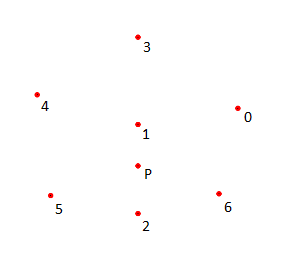
\includegraphics[width=0.4\linewidth]{rys3.png}
\end{figure} 

\subsection{Drzewo poszukiwań binarnych}
\qquad Do działania algorytmu konieczne jest uzyskiwanie informacji o najmniejszym elemencie zbioru aktualnie przecinanych krawędzi w czasie $O(log(n))$. Konieczne do tego jest użycie zmodyfikowanego drzewa poszukiwań binarnych. W przypadku tej implementacji użyte zostało drzewo AVL. W drzewie tym przechowywane są krawędzie aktualnie przecinające się z miotłą na podstawie rosnącej odległości punktu przecięcia od pewnego ustalonego punktu. Problematyczną kwestią jest fakt, że z każdym krokiem działania algorytmu miotła zmienia swoje położenie, co jest równoważne ze zmianą wartości punktów przecięcia miotły z krawędziami umieszczonymi na drzewie. Najprostszą możliwością zmiany wartości kluczy na drzewie jest zdjęcie z niego wszystkich elementów, zmiana ich wartości klucza i umieszczenie ponownie na drzewie. Nie jest to jednak optymalne podejście - taka operacja miałaby koszt $O(n*log(n))$. W rozwiązaniu tego zagadnienia pomaga fakt, że względna kolejność krawędzi umieszczonych na drzewie się nie zmienia - wraz z ruchem miotły elementy mogą być dodawane/usuwane, ale przez to, że krawędzie się nie przecinają nie może nastąpić ich zamiana kolejności w drzewie. Pozwala to na zastosowanie pewnej modyfikacji - dynamicznego ustalania wartości klucza dla każdego z elementów na drzewie. Oznacza to, że na drzewie przechowywane są krawędzie, ale bez przypisanych im wartości klucza. Te obliczane są za każdym razem, gdy wykonywana jest jakakolwiek operacja na drzewie i zależą od aktualnej pozycji miotły.

\noindent \qquad Kolejną kwestią związaną z drzewem są przypadki gdy podczas zamiatania trafiamy na punkt, z którego wychodzą dwie krawędzie, które muszą być dodane do drzewa. Gdyby chcieć je dodać z wartościami odległości jakie uzyskane są dla aktualnego stanu miotły, to obydwie krawędzie miałyby ten sam klucz, co może stwarzać problemy dla dalszego działania algorytmu. Aby ustalić odpowiedni porządek między tymi krawędziami na drzewie umieszczane one są na podstawie punktów przecięcia tych krawędzi z miotłą znajdującą się na następnej pozycji. W ten sposób unika się wystąpienia dwa razy tego samego klucza w drzewie, dalej zachowując odpowiednią kolejność elementów.

\subsection{Szczegóły implementacji algorytmu \textbf{czyWidoczny}}

\qquad Algorytm ten rozstrzyga, czy z punktu $P$ możliwe jest zobaczenie punktu $w_i$. Większa część jego implementacji jest prosta i polega jedynie na sprawdzeniu czy istnieje przecięcie dwóch odcinków. Sytuacja wygląda inaczej w przypadku pierwszego kroku, czyli sprawdzeniu czy $\overline{Pw_i}$ przechodzi przez środek wielokąta przy wierzchołku $w_i$. Sprawdzenie tego jest szczególnie konieczne, gdy zarówno punkt $P$ jak i $w_i$ należą do jednego wielokąta - jeżeli odcinek przechodzi wyłącznie przez jego środek, to nie jest przecinany przez inne krawędzie, dlatego konieczne jest ustalenie widoczności wierzchołka już na tym etapie.

\noindent \qquad Do rozwiązania tego problemu korzystamy z wyznaczenia położenia punktu $P$ względem prostych zawierających krawędzie wychodzące z $w_i$. Dwie proste przechodzące przez $w_i$ dzielą płaszczyznę na 4 części. To  w której części znajduje się punkt $P$ (przypadki współliniowe obsługiwane są osobno) determinuje czy $\overline{Pw_i}$ przechodzi przez środek wielokąta. Wpływ na to która część daje dany wynik ma kąt wewnętrzny wielokąta przy $w_i$, jeżeli kąt jest wypukły, to tylko dla położenia $P$ w jednej z części odcinek $\overline{Pw_i}$ będzie przechodził przez środek wielokąta. Dla kąta wklęsłego taki przypadek występuje dla trzech części. W implementacji tej metody dodatkowo konieczne było określenie po której stronie układu trzech punktów (punktu $w_i$ i jego sąsiadów) znajduje się wnętrze wielokąta. Konieczne do tego było wyznaczenie kolejności w jakiej został zadany wielokąt (zgodnie / przeciwnie do ruchu wskazówek zegara). Z takimi informacjami wszystkie pozostałe obliczenia (zarówno wypukłości / wklęsłości kąta, jak i położenia $P$ względem prostych) możliwe były przy użyciu wyznacznika.

\begin{figure}[ht] % tutaj trzeba wrzucić rysunki z tymi dwoma przypadkami ahh
\caption{}
\centering
\begin{subfigure}{.5\textwidth}
\centering
\caption{Kąt wypukły przy wierzchołku $w_i$. Dla P leżącego \newline w części 4 prosta $\overline{Pw_i}$ przechodzi przez środek wielokąta.}
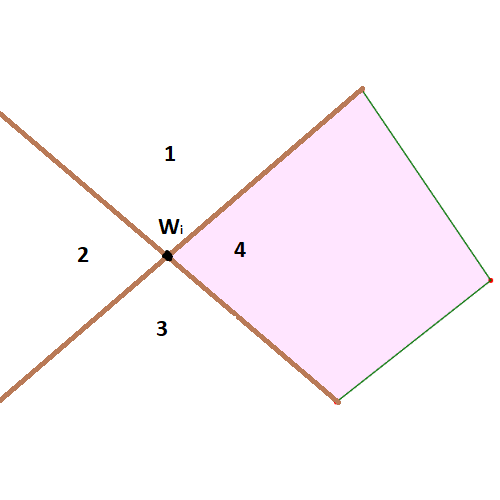
\includegraphics[width=.75\linewidth]{rys4a.png}
\end{subfigure}%
\begin{subfigure}{.5\textwidth}
\centering
\caption{Kąt wklęsły przy wierzchołku $w_i$. Dla P leżącego w częściach 1, 3, 4 prosta $\overline{Pw_i}$ przechodzi przez środek wielokąta.}
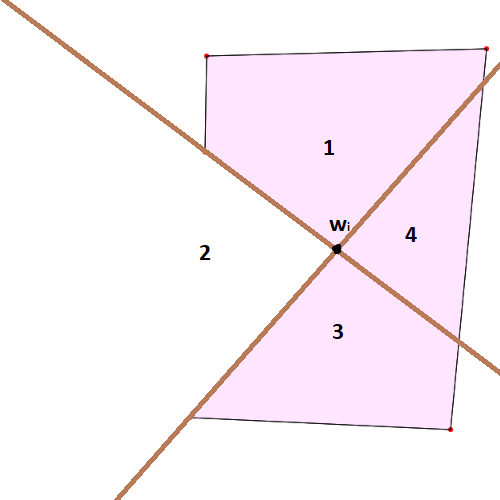
\includegraphics[width=.75\linewidth]{rys4b.png}
\end{subfigure}%
\end{figure}


\section{Wizualizacja graficzna}

\subsection{Podstawowa wizualizacja danych wejściowych i grafu widoczności}

\qquad Program stworzony na potrzeby wizualizacji algorytmu napisany został w języku JavaScript i jest uruchamiany za pośrednictwem przeglądarki internetowej. Program umożliwia wczytywanie zbioru wielokątów z pliku i zapisywanie wynikowego grafu widoczności do pliku (te i inne funkcje opisane są szczegółowiej w dokumentacji technicznej). Poza podstawową funkcją rysowania grafu widoczności program pozwala na zobaczenie działania funkcji \textbf{widoczneWierzchołki} dla wybranego wierzchołka z wejściowych danych (Rysunek 2.), a także dla punktu wskazywanego aktualnie przez myszkę na ekranie (Rysunek 5.) - w tym przypadku mogą wystąpić błędy programu, gdy myszka znajdzie się wewnątrz wielokąta, bądź na jego punktach czy krawędziach.

\begin{figure}[ht]
\centering
\caption{\centering Przykładowe działanie algorytmu \textbf{widoczneWierzchołki} dla pozycji wskazanej przez myszkę.}
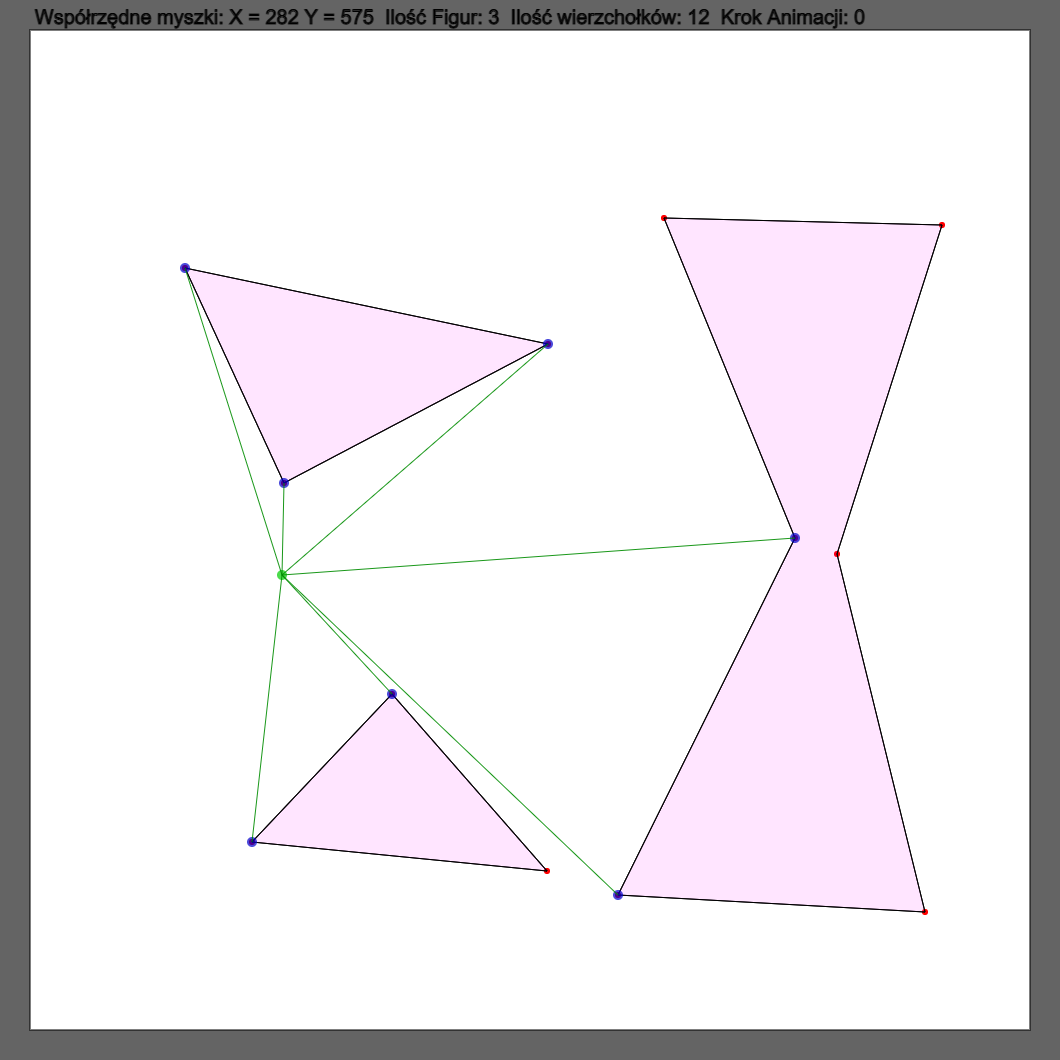
\includegraphics[width=0.5\linewidth]{rys5.png}
\end{figure} 

\noindent \qquad W podstawowej części aplikacji przyjęty jest następujący schemat kolorów:
\begin{itemize}
\item różowy/błękitny - wnętrze zadanego wielokąta (przeszkody)
\item czerwony punkt - wierzchołek wielokąta
\item zielony punkt - punkt z którego przeprowadzany jest algorytm \textbf{widoczneWierzchołki}
\item niebieski punkt - wierzchołek wielokąta, który jest widoczny podczas działania algorytmu \textbf{widoczneWierzchołki}
\item zielony odcinek - oznacza, że dwa punkty będące jego końcami ``widzą się wzajemnie''
\end{itemize}

\subsection{Animacja algorytmu \textbf{grafWidoczności}}

\qquad Program pozwala na wyświetlenie kolejnych kroków głównej pętli programu, czyli pokazanie nakładających się na siebie wyników działania algorytmu \textbf{widoczneWierzchołki}. 




\begin{figure}[p]
\caption{Kolejne kroki w animacji algorytmu \textbf{grafWidoczności}}
    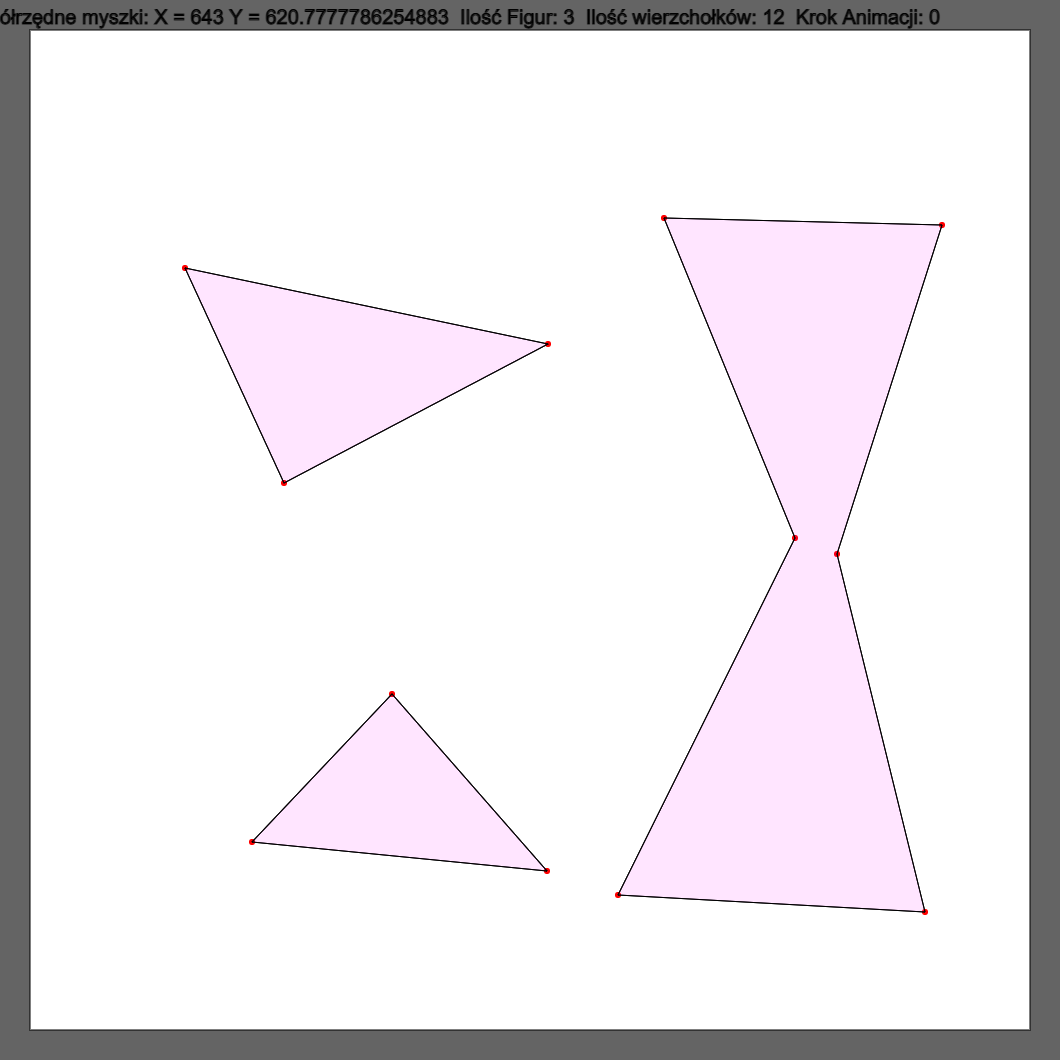
\includegraphics[width=.32\textwidth]{agw1.png}\hfill
    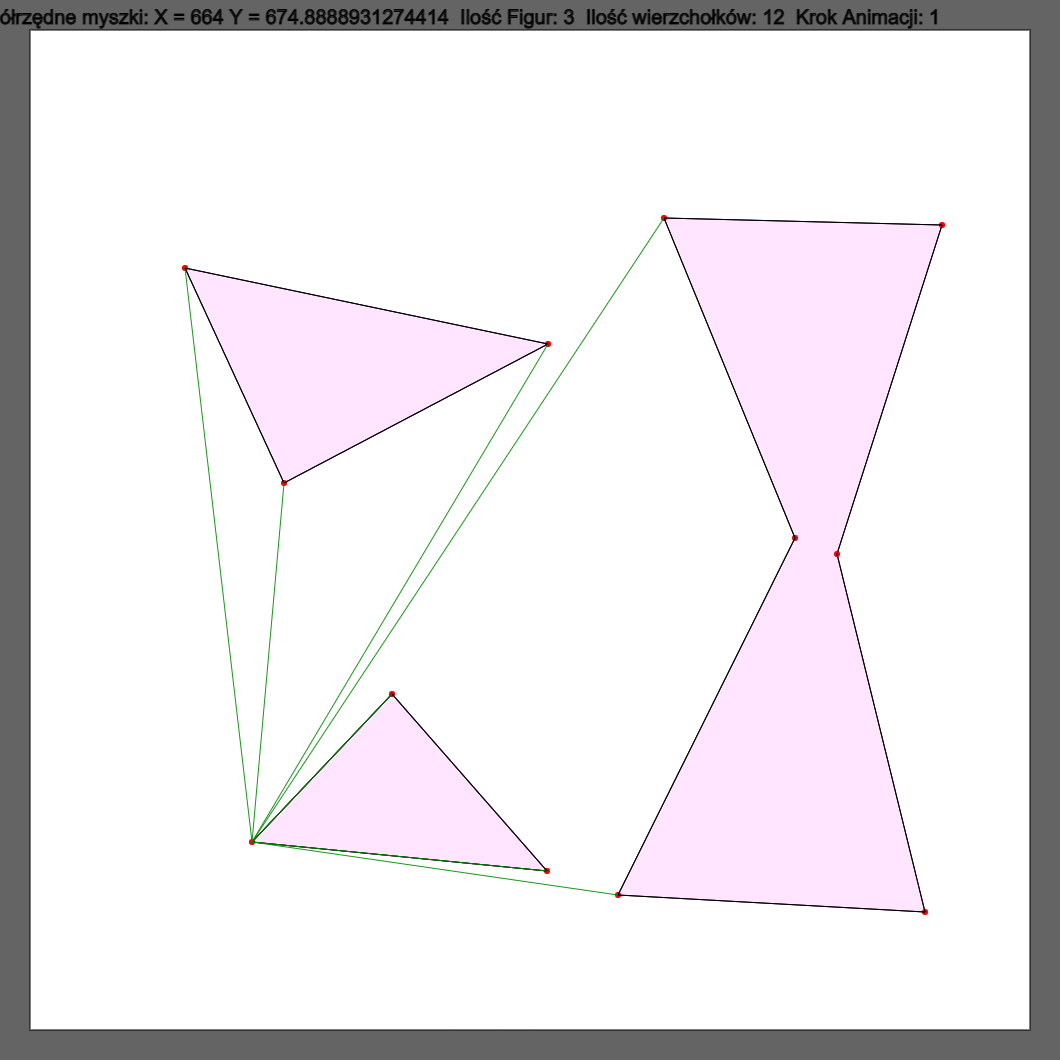
\includegraphics[width=.32\textwidth]{agw2.png}\hfill
    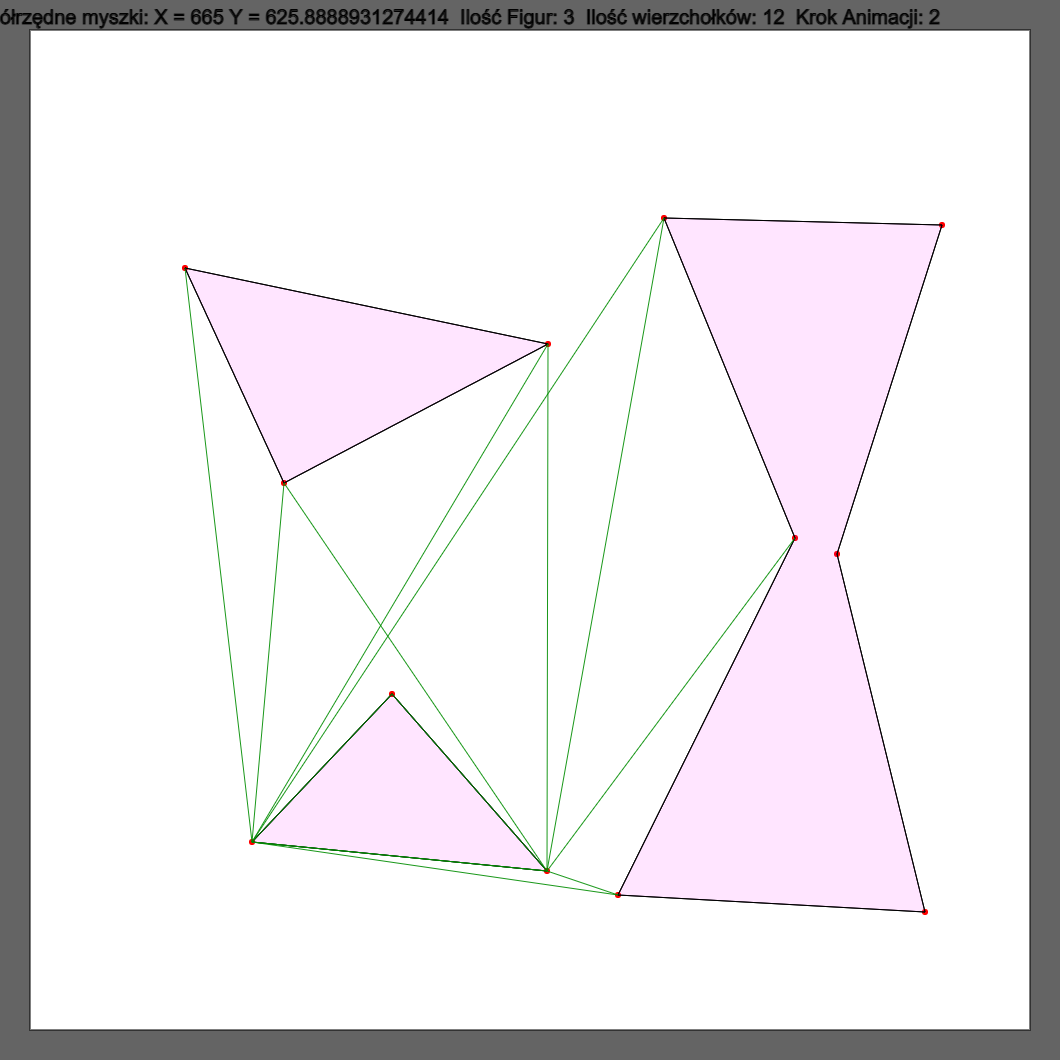
\includegraphics[width=.32\textwidth]{agw3.png}
    \\[\smallskipamount]
    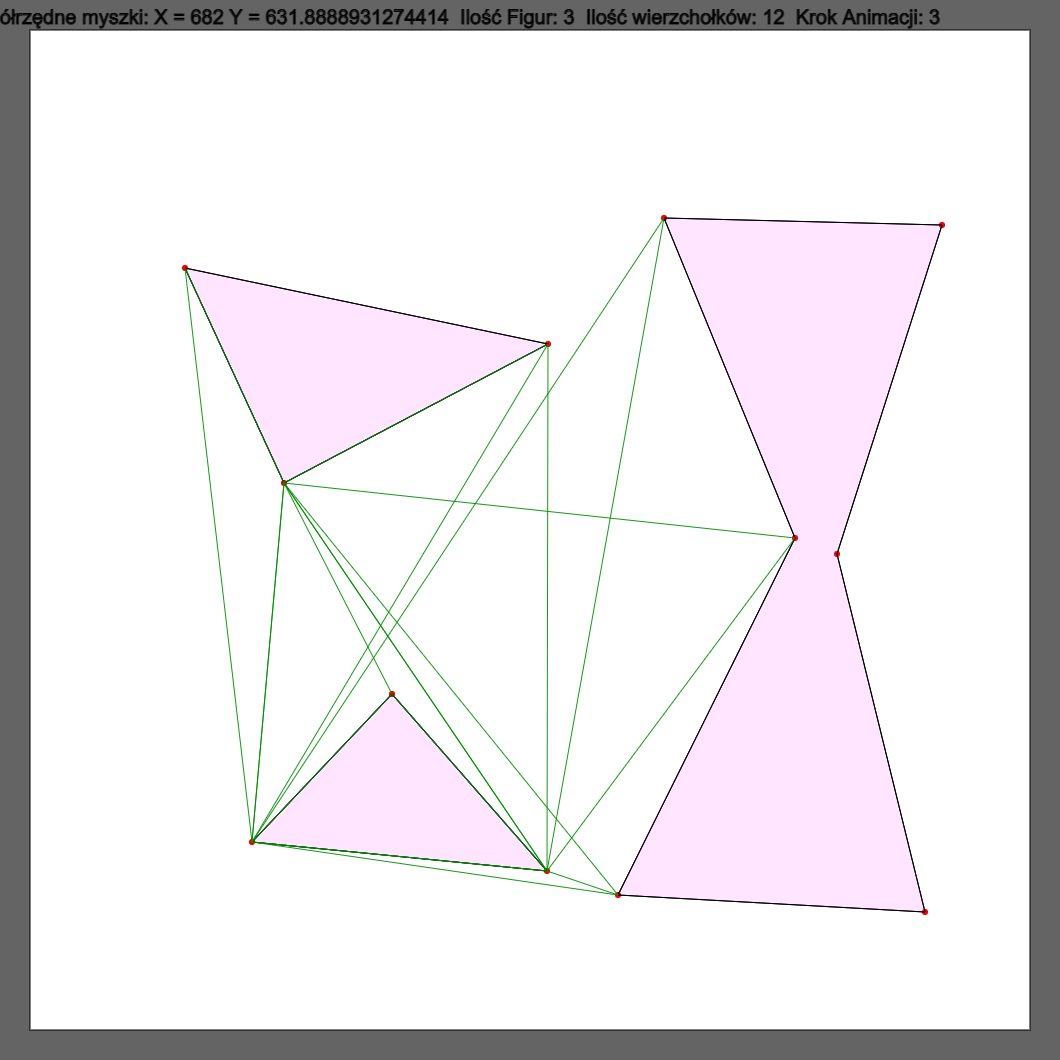
\includegraphics[width=.32\textwidth]{agw4.png}\hfill
    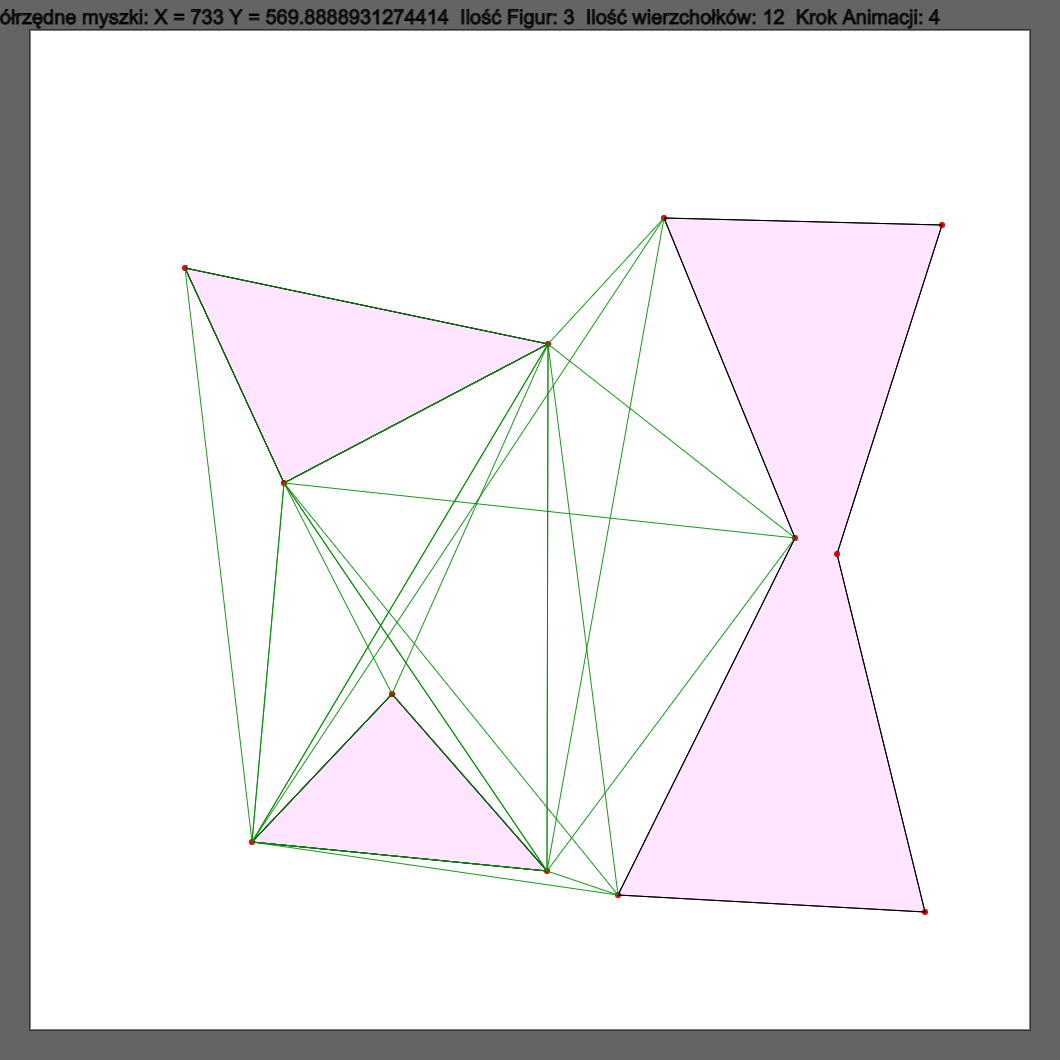
\includegraphics[width=.32\textwidth]{agw5.png}\hfill
    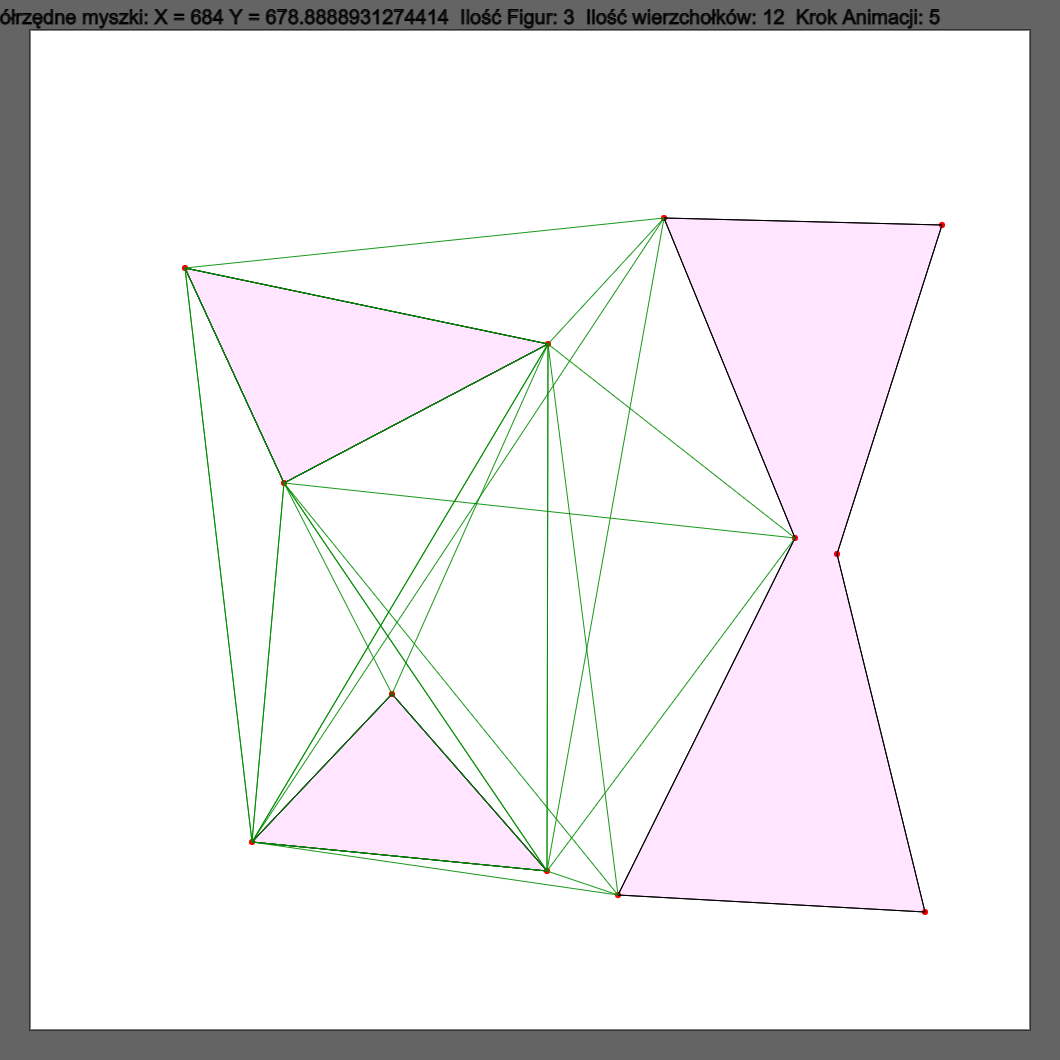
\includegraphics[width=.32\textwidth]{agw6.png}
    \\[\smallskipamount]
    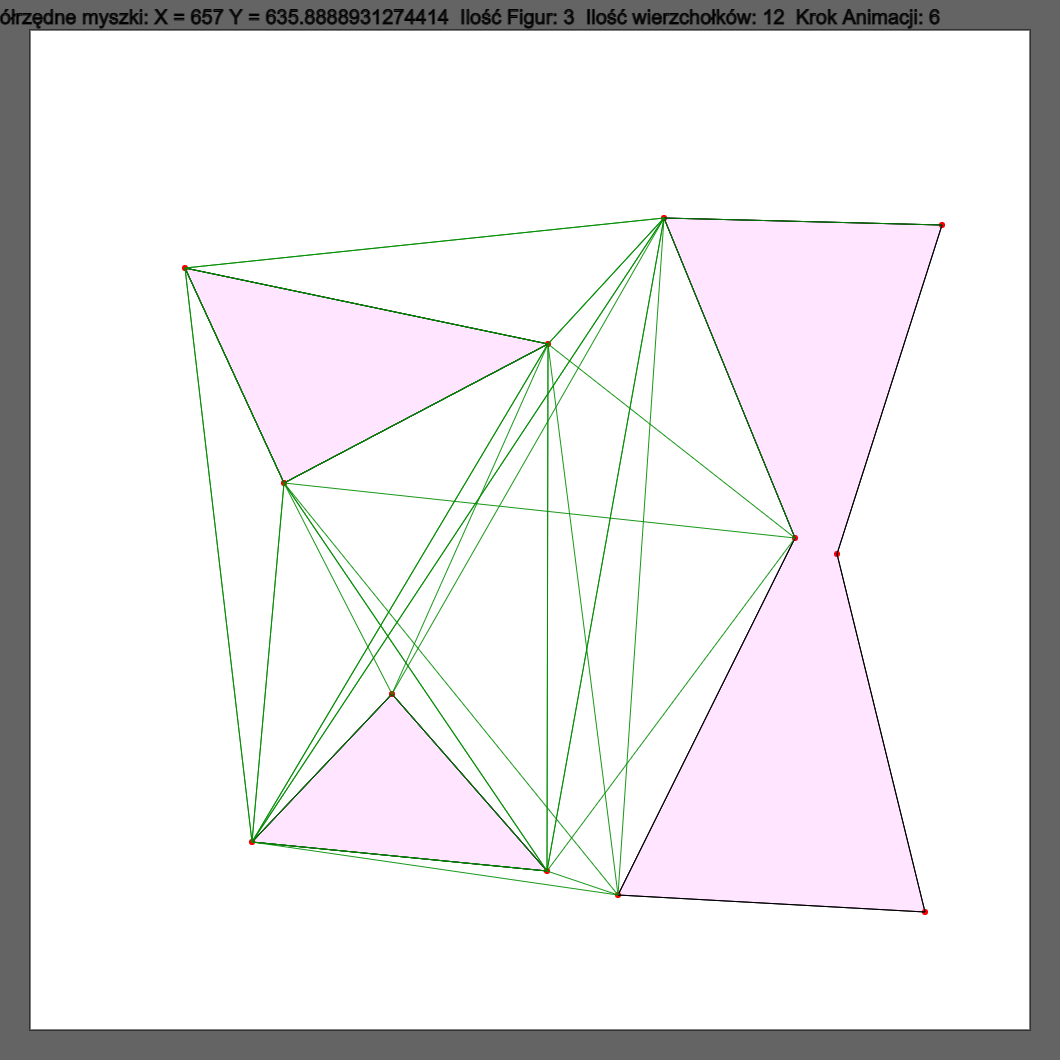
\includegraphics[width=.32\textwidth]{agw7.png}\hfill
    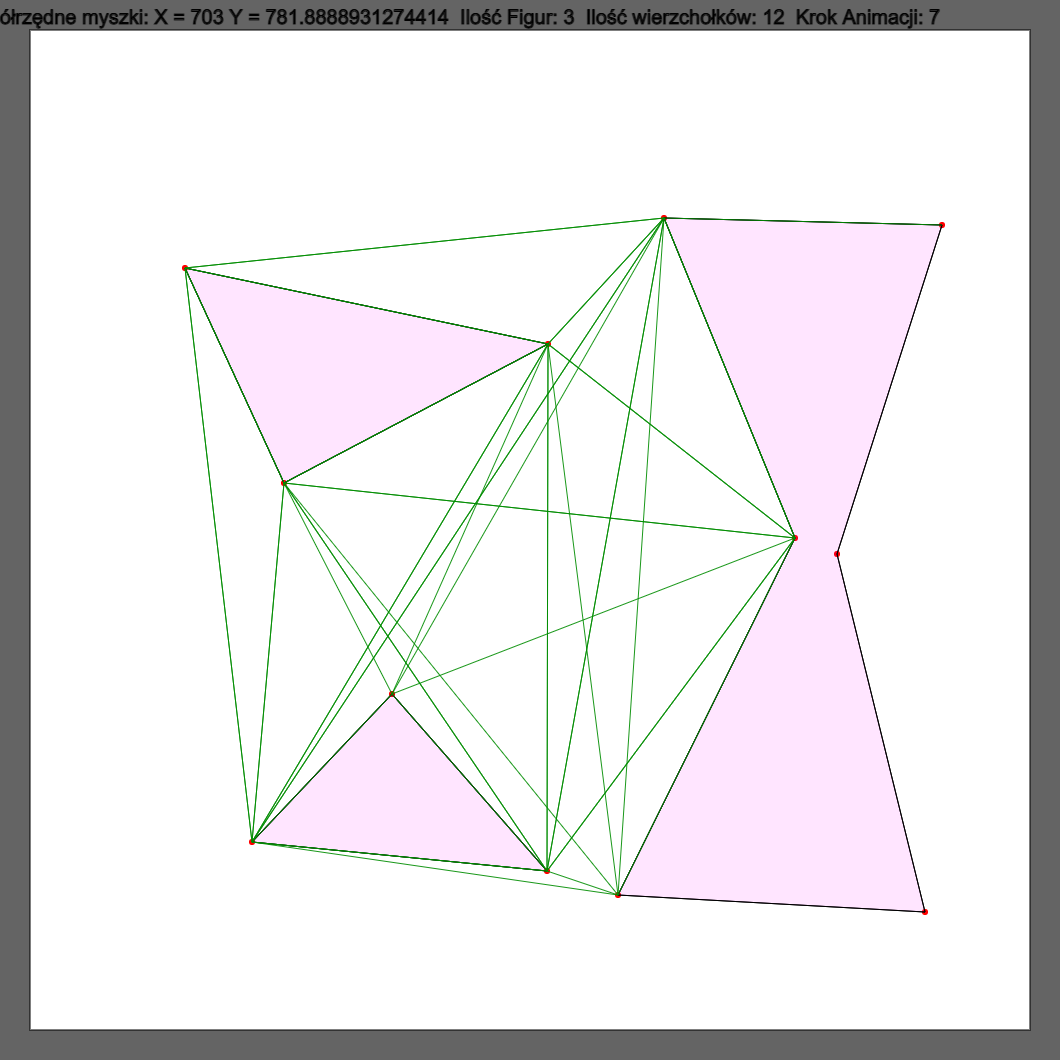
\includegraphics[width=.32\textwidth]{agw8.png}\hfill
    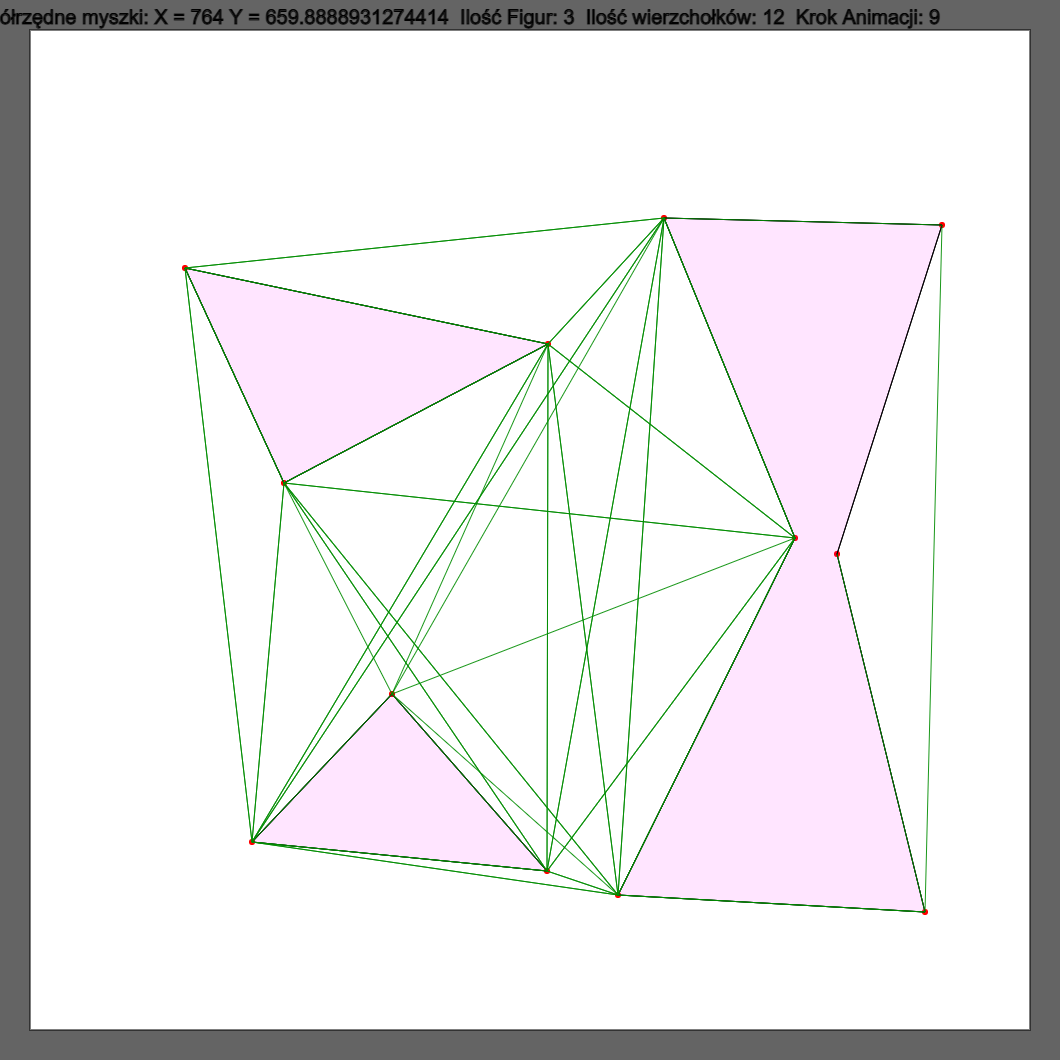
\includegraphics[width=.32\textwidth]{agw9.png}
    
\end{figure}
\newpage

\subsection{Animacja algorytmu \textbf{widoczneWierzchołki}}
\qquad Najistotniejszym wizualnym elementem programu jest możliwość wyświetlenia krok po kroku animacji algorytmu zamiatania \textbf{widoczneWierzchołki}. Wizualizacja uwzględnia aktualną pozycję miotły i krawędzie aktualnie przechowywane na drzewie. Jeżeli występują przecięcia uniemożliwiające uznanie danego wierzchołka za widoczny, to wizualizacja także to sygnalizuje. Na wizualizacji nie jest prezentowane dokładne działanie algorytmu \textbf{czyWidoczny} dla przypadków punktów współliniowych. Przyjęty schemat kolorystyczny:

\begin{itemize}
\item niebieski odcinek - miotła w swoim aktualnym położeniu
\item szare krawędzie wielokątów - krawędzie przebywające aktualnie na drzewie
\item mały zielony punkt - punkt z którego przeprowadzany jest algorytm \textbf{widoczneWierzchołki}
\item czerwona krawędź wielokąta - krawędź będąca najmniejszą w drzewie, z którą sprawdzane jest przecięcie miotły
\item większy zielony punkt - punkt przecięcia miotły z czerwoną krawędzią
\item większy czerwony punkt - punkt uznany z widoczny w danym kroku
\item niebieski punkt - wierzchołek wielokąta, który jest widoczny podczas działania algorytmu \textbf{widoczneWierzchołki}
\item zielony odcinek - oznacza, że dwa punkty będące jego końcami ``widzą się wzajemnie''
\end{itemize}

\begin{figure}[p]
\caption{Poszczególne kroki algorytmu \textbf{widoczneWierzchołki}}
    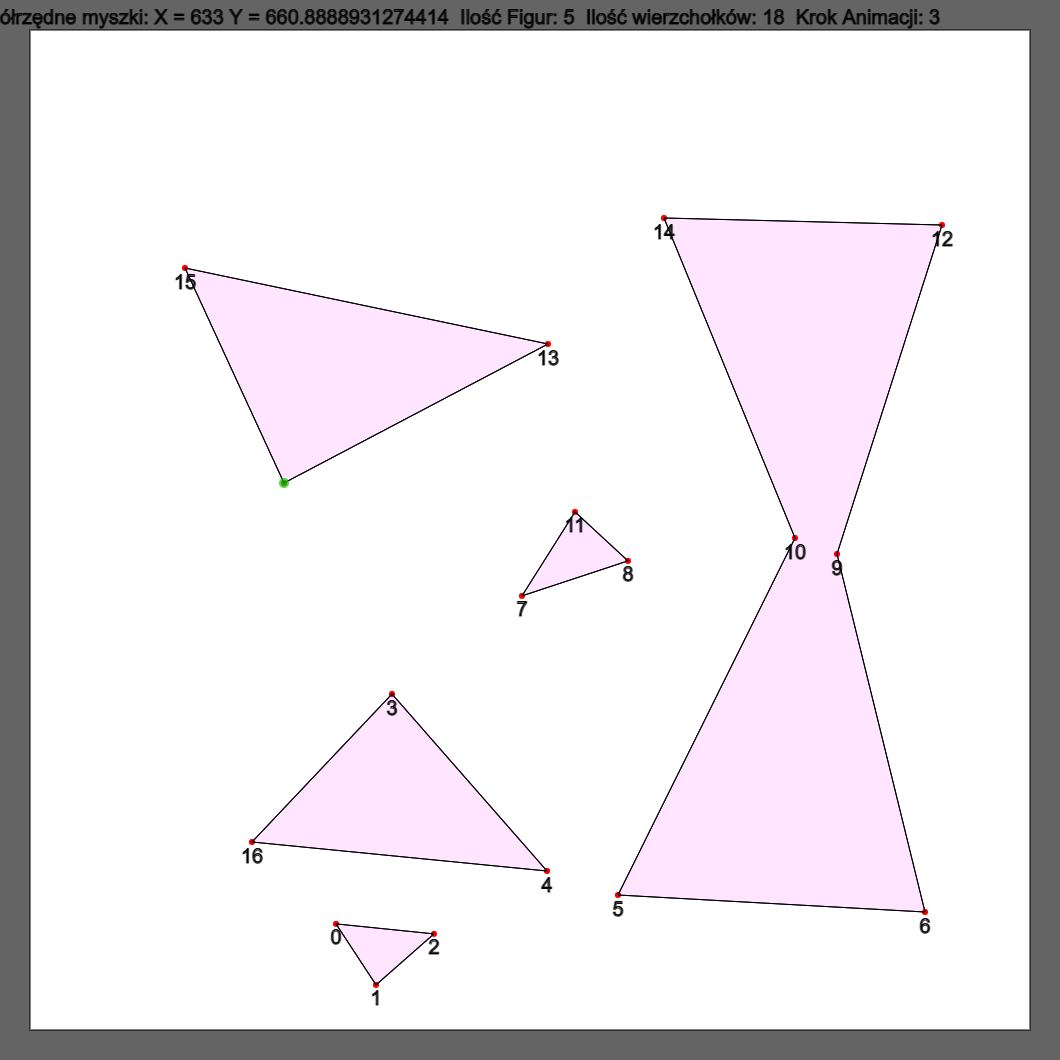
\includegraphics[width=.32\textwidth]{ww2.png}\hfill
    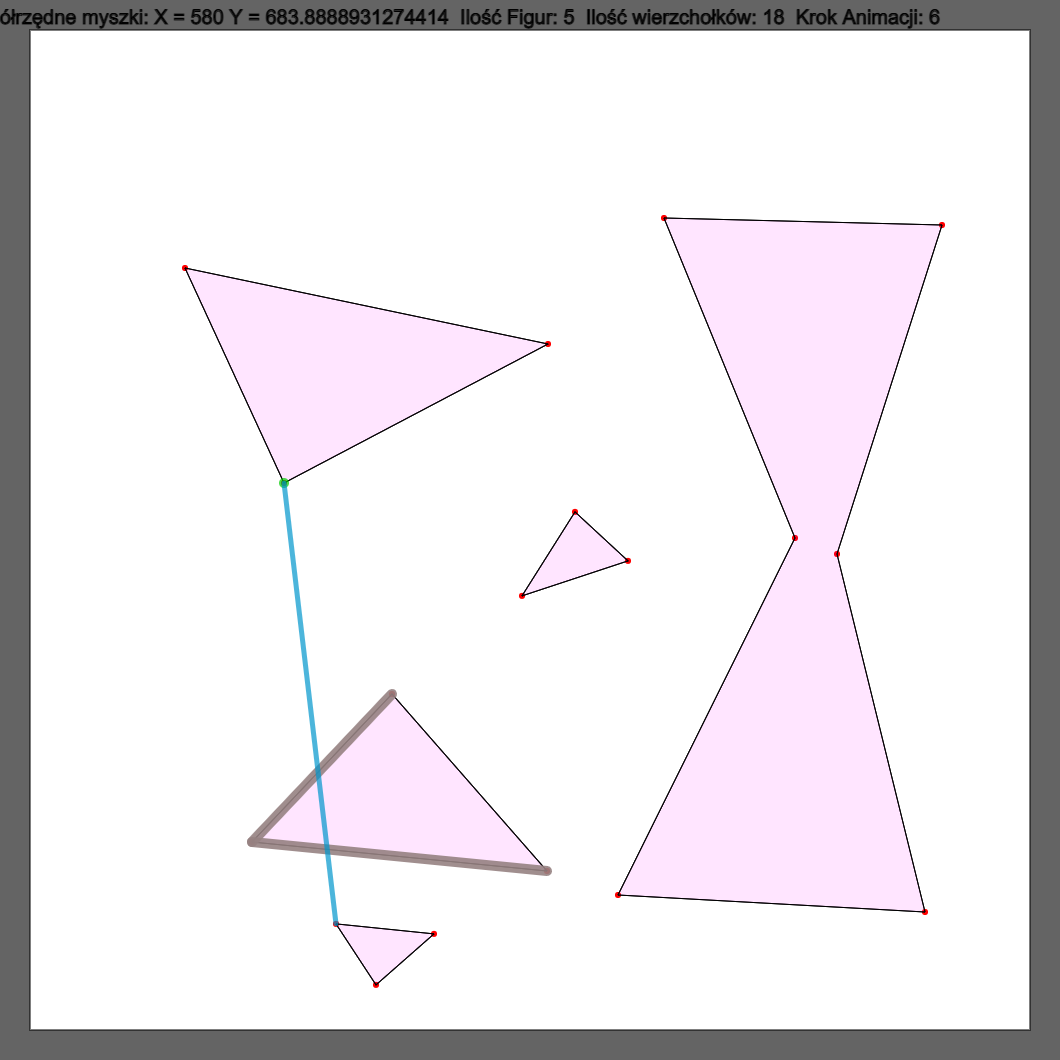
\includegraphics[width=.32\textwidth]{ww3.png}\hfill
    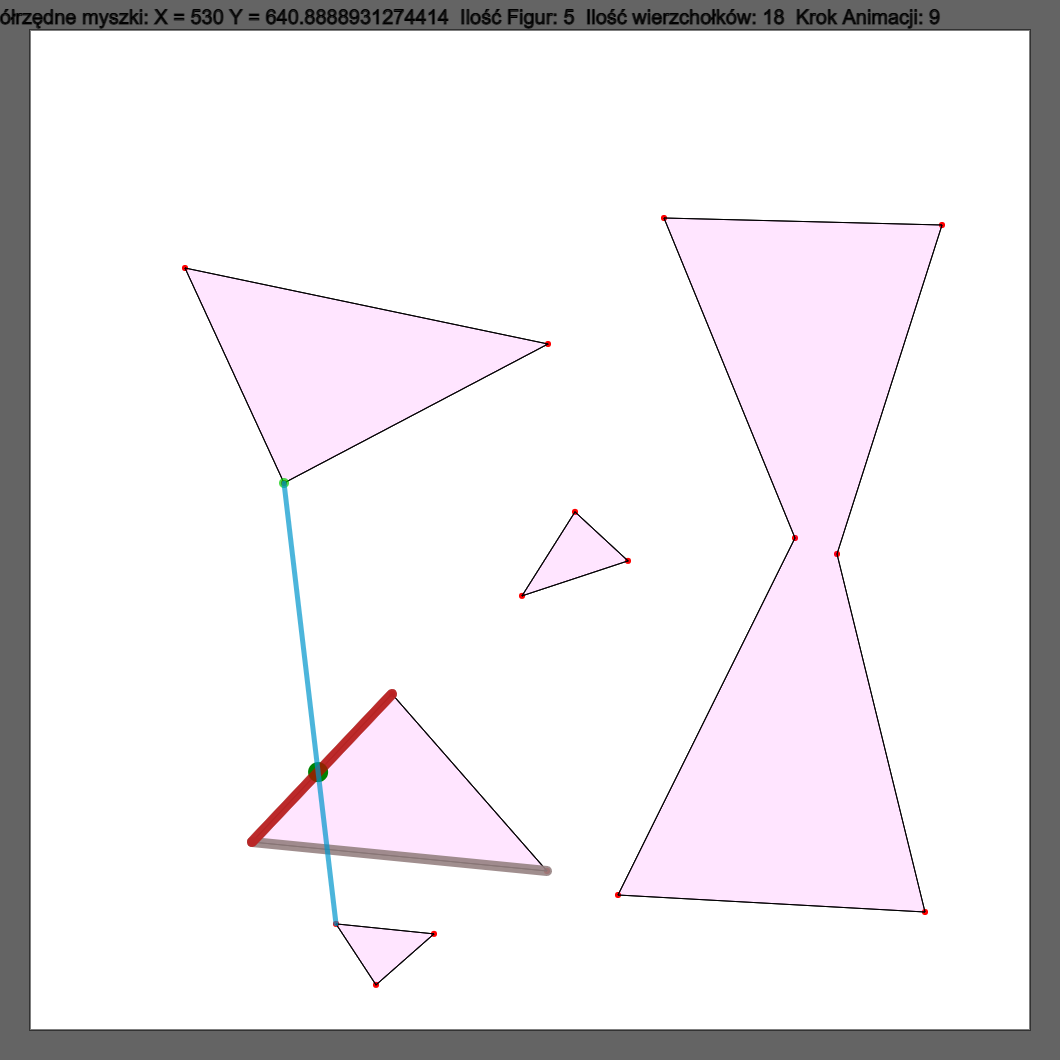
\includegraphics[width=.32\textwidth]{ww4.png}
    \\[\smallskipamount]
    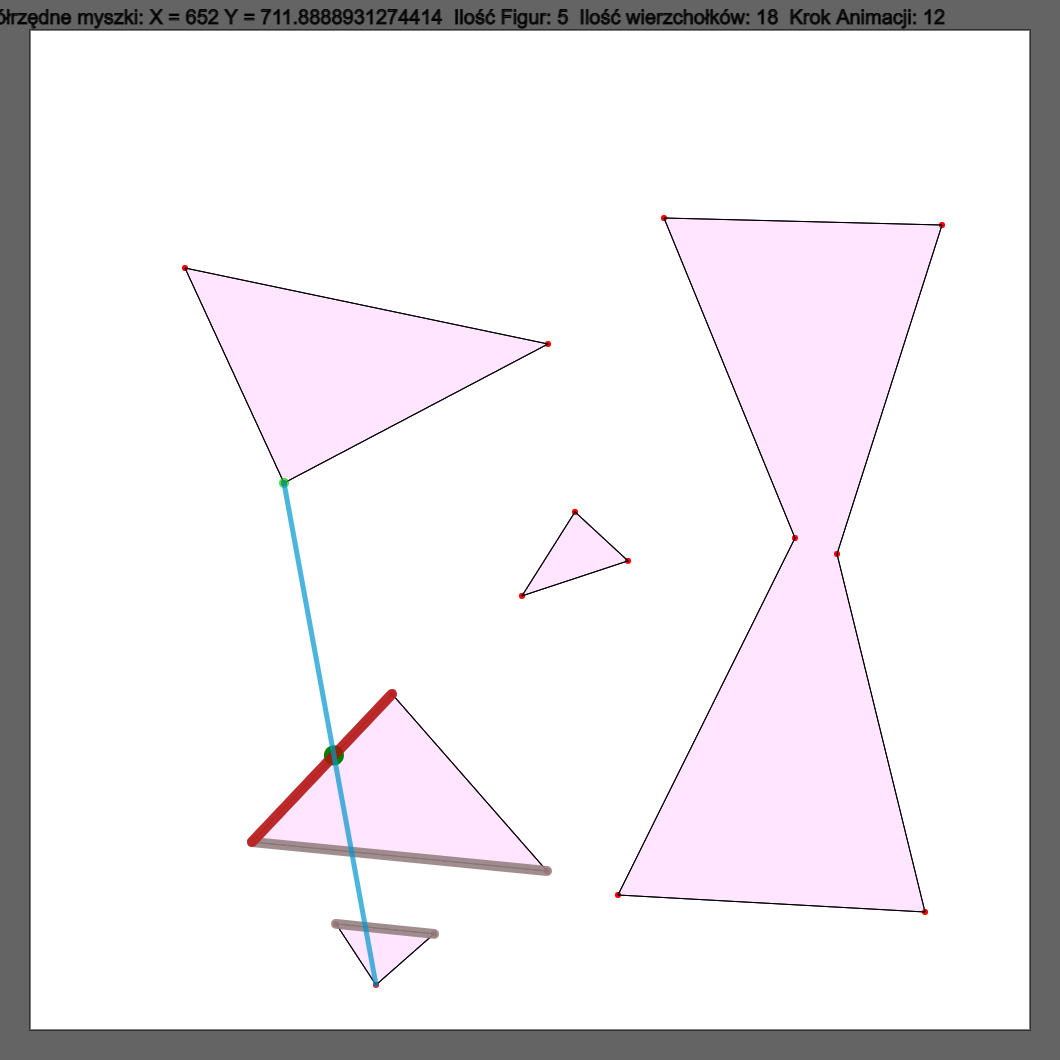
\includegraphics[width=.32\textwidth]{ww5.png}\hfill
    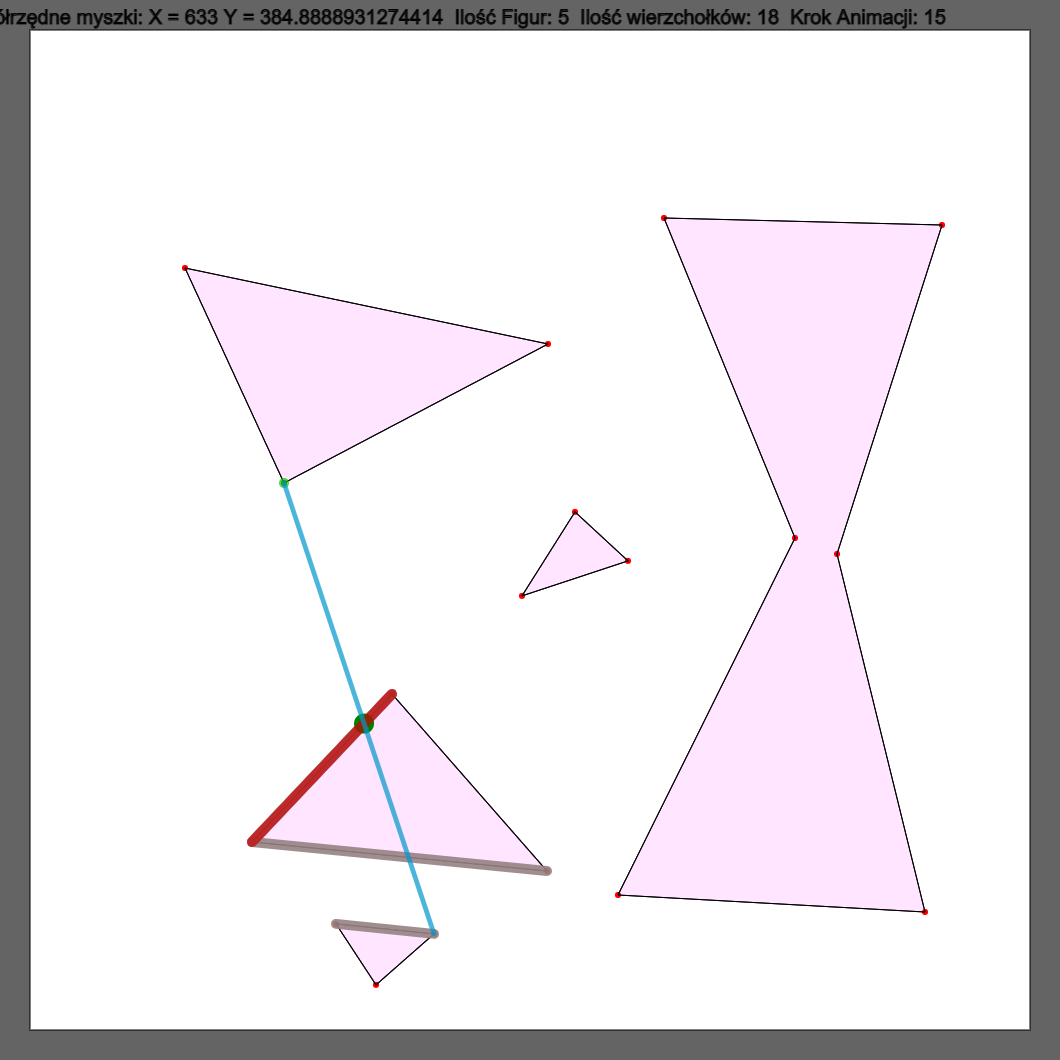
\includegraphics[width=.32\textwidth]{ww6.png}\hfill
    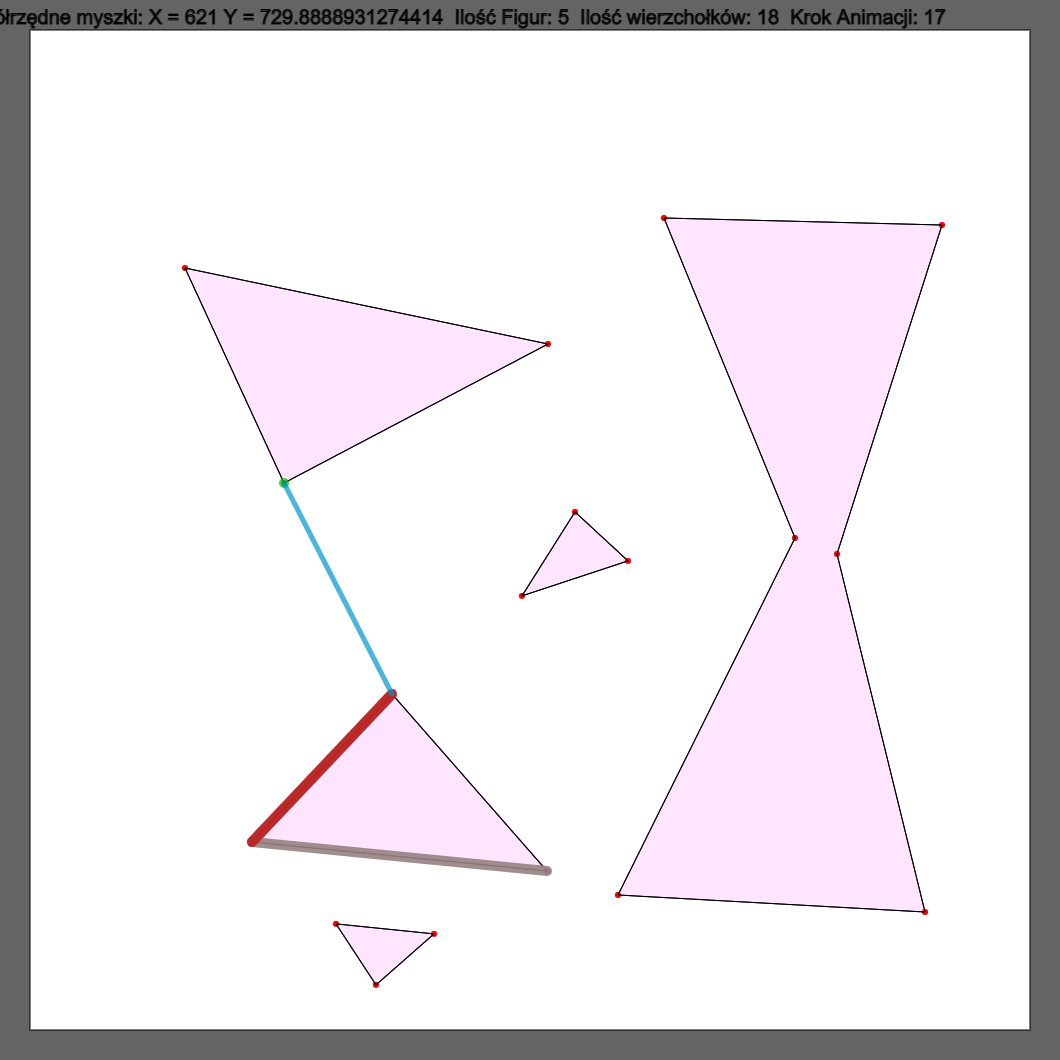
\includegraphics[width=.32\textwidth]{ww7.png}
    \\[\smallskipamount]
    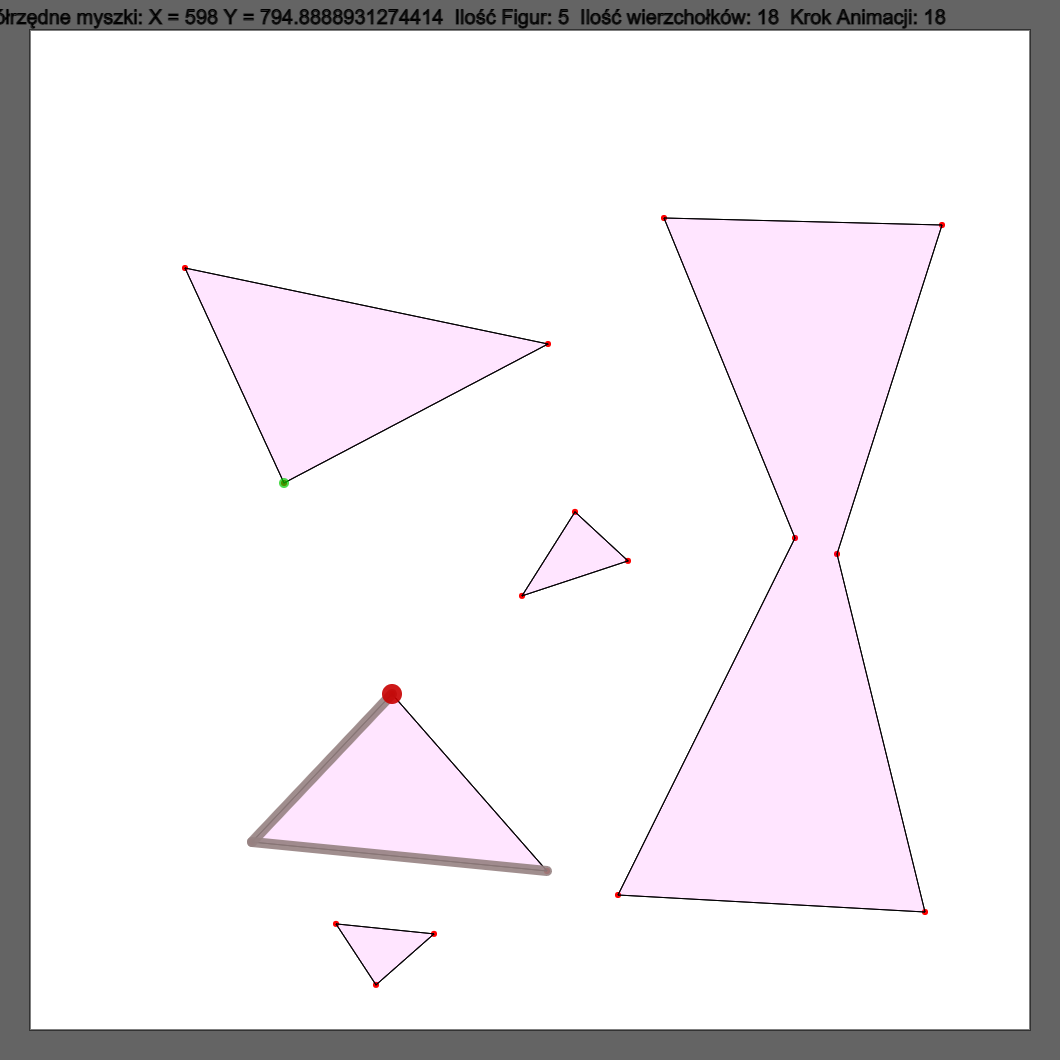
\includegraphics[width=.32\textwidth]{ww8.png}\hfill
    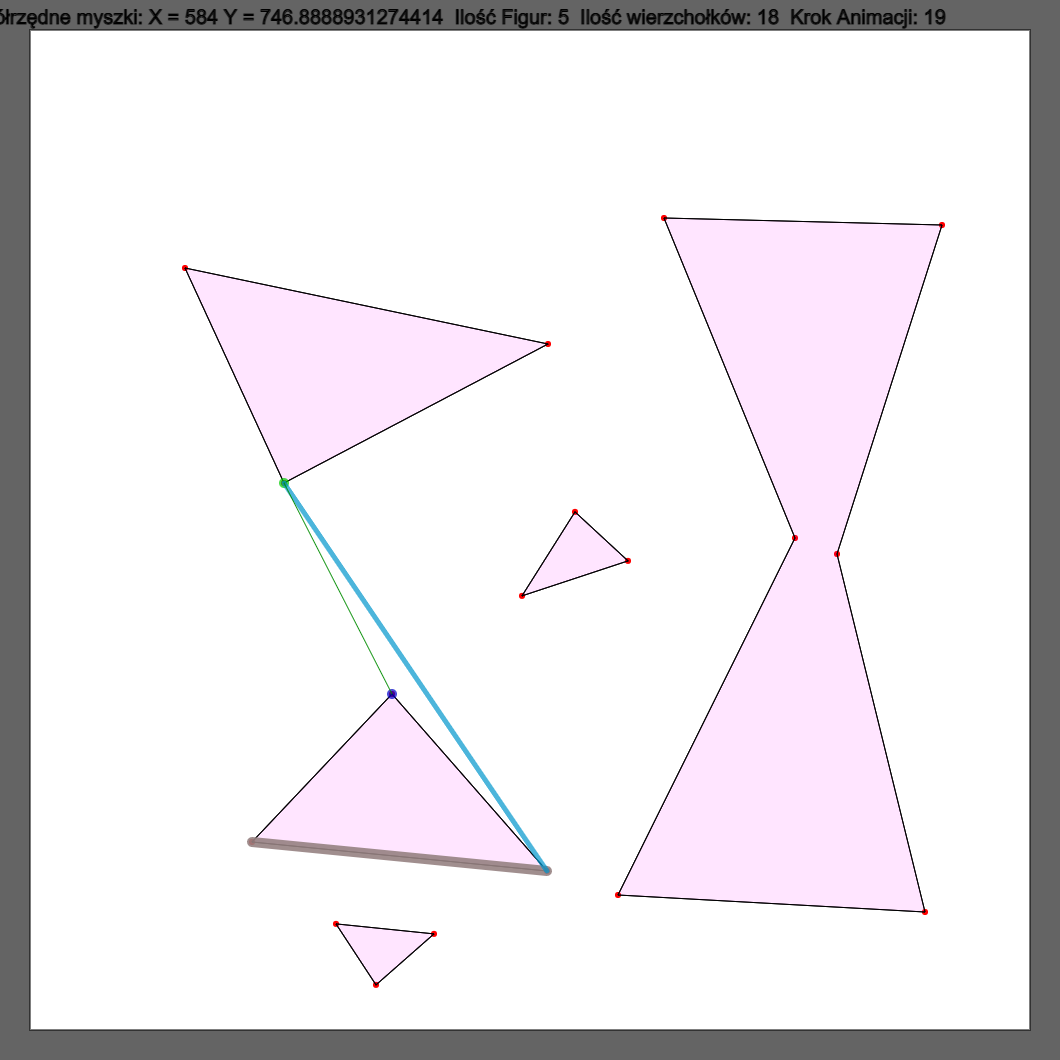
\includegraphics[width=.32\textwidth]{ww9.png}\hfill
    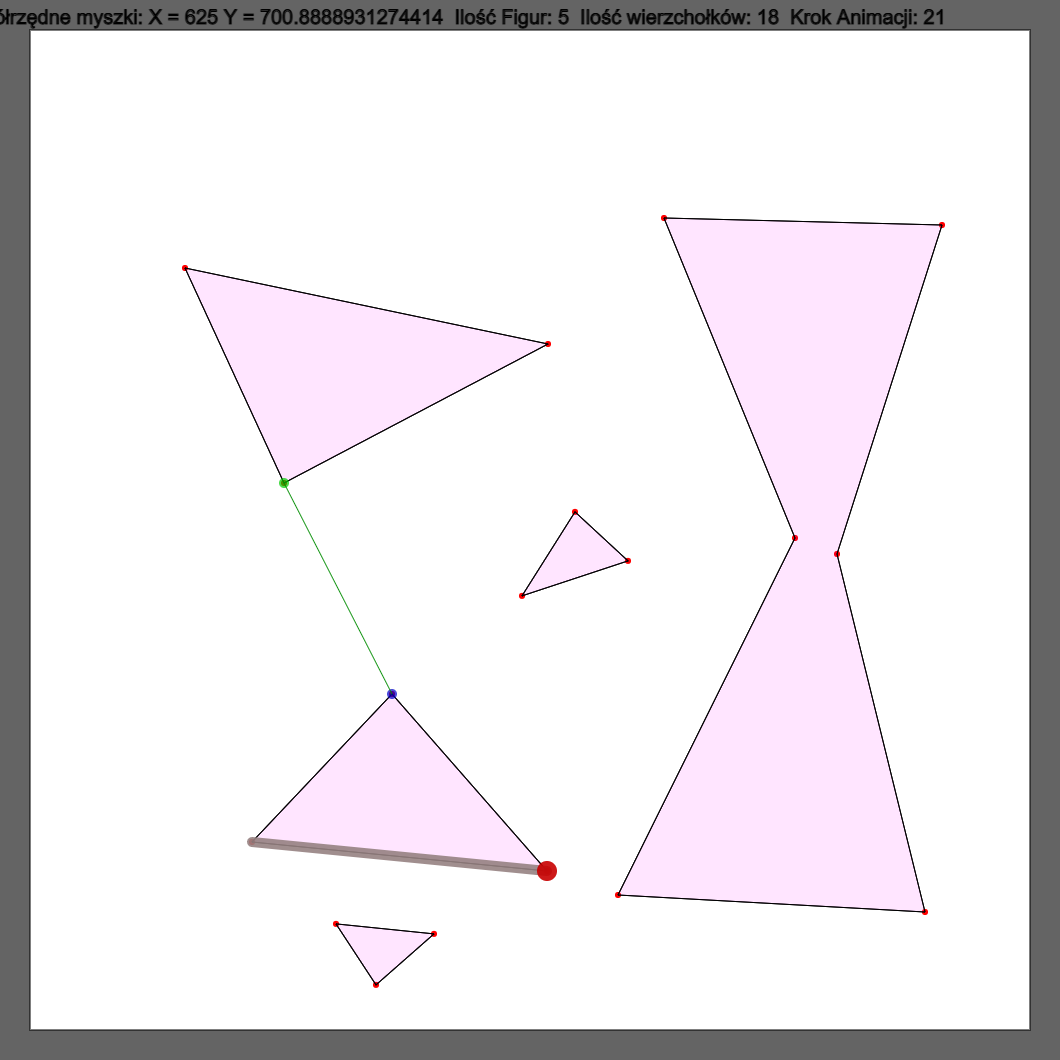
\includegraphics[width=.32\textwidth]{ww10.png}
    \\[\smallskipamount]
    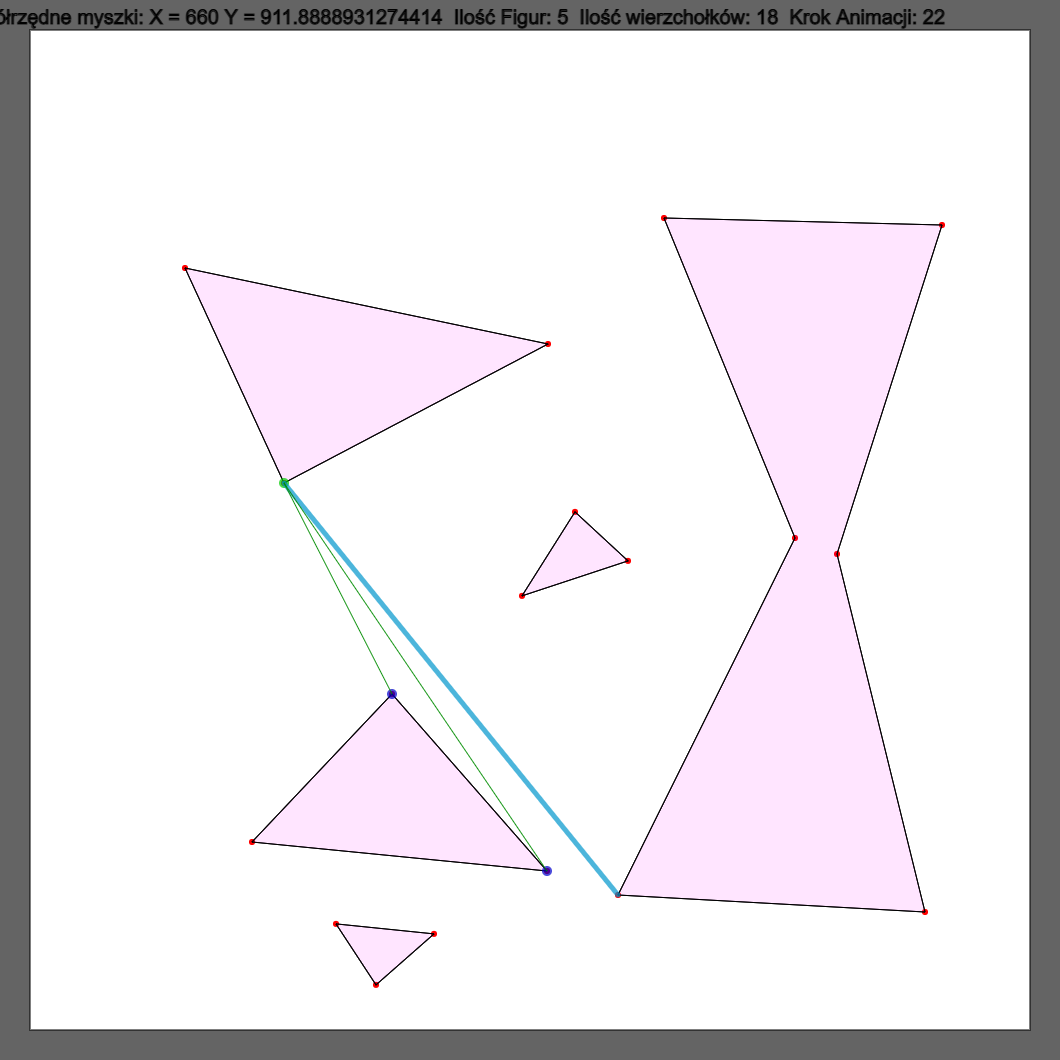
\includegraphics[width=.32\textwidth]{ww11.png}\hfill
    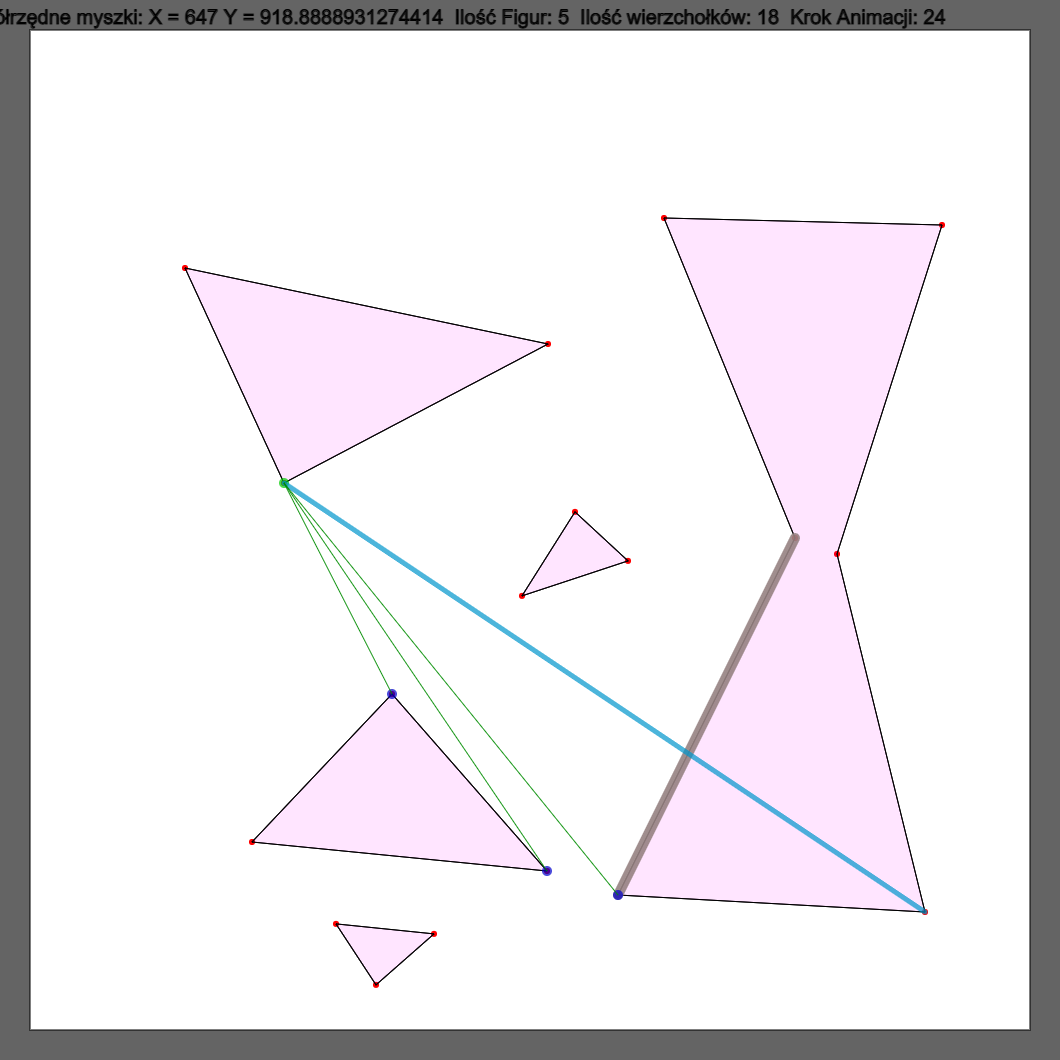
\includegraphics[width=.32\textwidth]{ww12.png}\hfill
    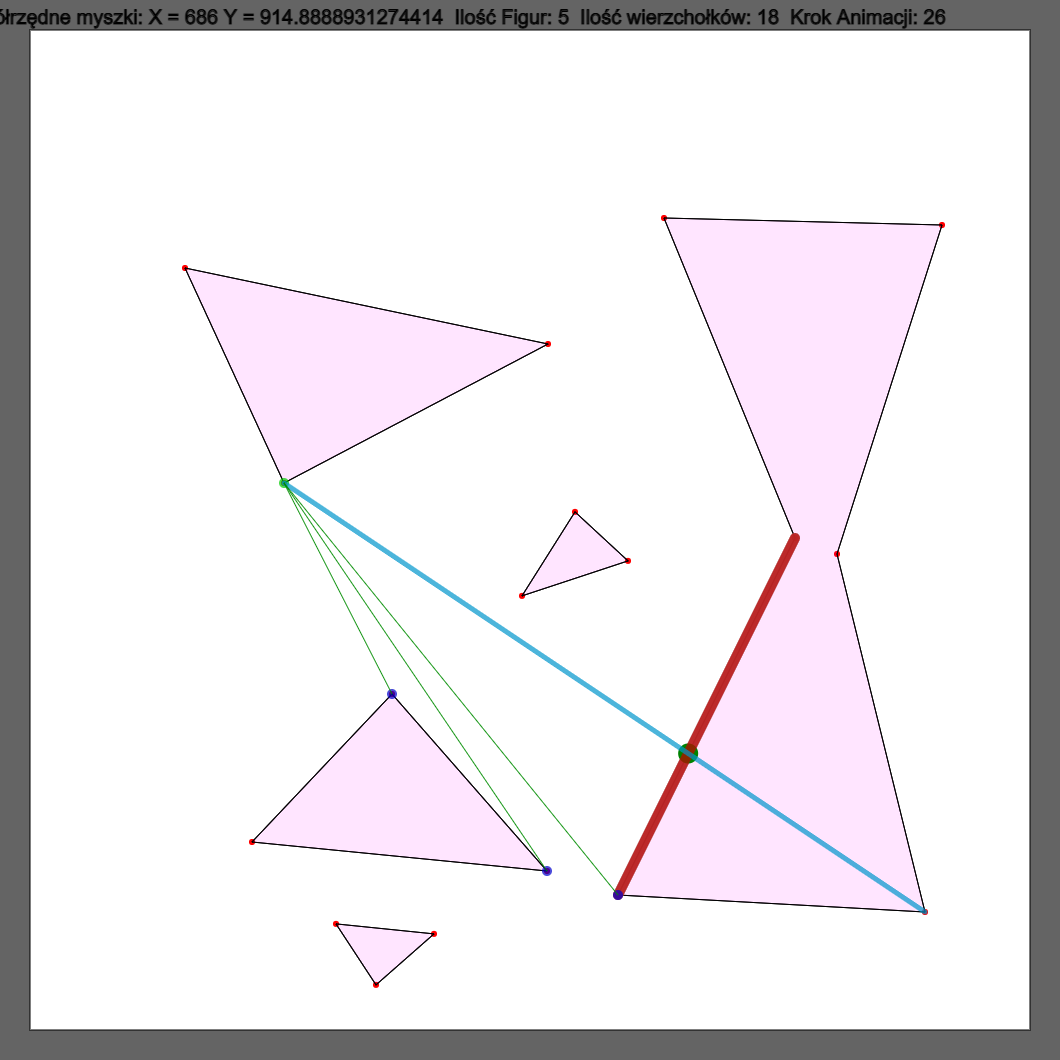
\includegraphics[width=.32\textwidth]{ww13.png}
    
\end{figure}


% tutaj wrzucić z 4 / 5 zestawów danych które pokazują wyniki dla przykładów ze współliniowoąscią itp, jak jakieś ciekawsze są to opisać je

% tutaj graficzki z animacją widocznych wierzchołków 

\section{\texorpdfstring{Porównanie z naiwnym algorytmem $O(n^3)$}{}} 

\qquad W celu sprawdzenia działania prezentowanego algorytmu oraz jego poprawności zaimplementowany został naiwny algorytm o złożoności $O(n^3)$. Jego działanie polega na sprawdzeniu każdej pary punktów i każdej krawędzi, co daje informacje o ich wzajemnej widoczności. Przeprowadzone porównanie polegało na zmierzeniu czasów wykonania obydwu algorytmów dla danych wejściowych o różnym rozmiarze, a jego wyniki prezentowane są w tabeli poniżej.

\begin{table}[h]
\caption{Czasy obliczania grafu widoczności w sekundach, w zależności od algorytmu i ilości punktów w danych wejściowych}
\centering
\begin{tabular}{cccccccc}
                      & 10    & 50    & 100   & 250   & 500    & 750    & 1000    \\ \hline
$O(n^2*log(n))$                & 0.002 & 0.059 & 0.336 & 2.586 & 8.156  & 19.205 & 40.091  \\ \hline
$O(n^3)$             & 0.002 & 0.083 & 0.525 & 8.707 & 35.263 & 74.822 & 175.035
\end{tabular}
\end{table}

\noindent \qquad  Aplikacja stworzona do wizualizacji algorytmu umożliwia dla każdego zestawu danych przeprowadzić porównanie czasowe między dwoma metodami obliczania grafu widoczności. Służy do tego odpowiedni przycisk. Implementowany algorytm zgodnie z oczekiwaniami osiąga lepsze wyniki w teście wydajnościowym. Podczas testów zdarzały się jednak przypadki, gdy dla małych danych wejściowych (liczba wierzchołków mniejsza od 30) algorytm naiwny był szybszy. Ma to związek najprawdopodobniej z faktem, że algorytm zamiatania wymaga dodatkowej pracy jak tworzenie miotły, czy obliczenia wykonywane na elementach drzewa, a także sprawdzanie widoczności, co chociaż nie zmienia złożoności algorytmu, to wpływa na jego czas działania.

\newpage

\section{Przykładowe wyniki działania algorytmu}

\subsection{``Kwadraty''}
\qquad Istotnym zestawem danych, na którym była testowana poprawność algorytmu był zbiór równo rozłożonych kwadratów, o takich samych wymiarach, jak i odległościach między sobą. Na tym zbiorze testowane były poprawność działania sortowania, a także wszystkich wariantów algorytmu \textbf{czyWidoczny}, ze względu na różne rodzaje współliniowości punktów.


\begin{figure}[h]
\centering
\caption \centering{Zestaw danych ``Kwadraty'', przykład funkcji \textbf{widoczneWierzchołki} oraz wynikowy graf widoczności}
    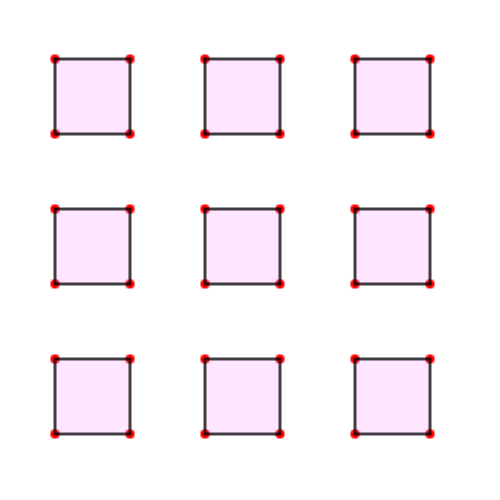
\includegraphics[width=.32\textwidth]{rys10.png}\hfill
    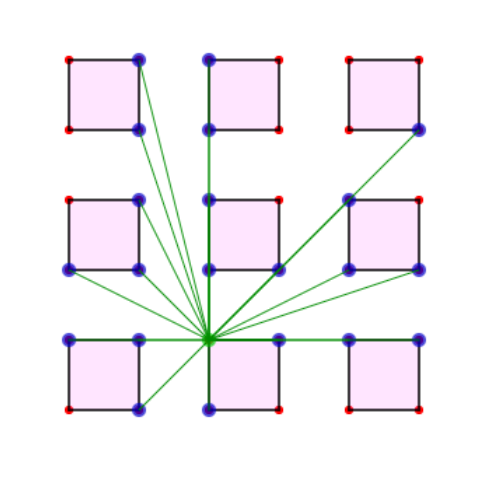
\includegraphics[width=.32\textwidth]{rys8.png}\hfill
    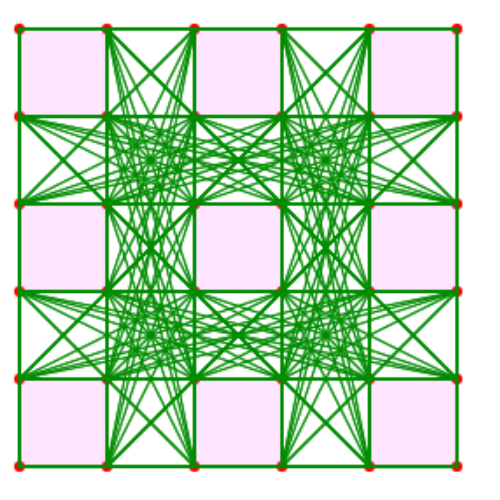
\includegraphics[width=.32\textwidth]{rys9.png}
\end{figure}

\subsection{Duży zestaw danych}
\qquad Zestawy danych mające wiele punktów, okazały się bardzo użyteczne pod kątem znajdowania problemów w działaniu algorytmu. Duża gęstość punktów na takich danych pozwala na uzyskanie różnego rodzaju przypadków związanych z np. współliniowością punktów czy odcinkami pionowymi i poziomymi, a także z różnymi zachowaniami drzewa. W fazie testowania programu wykrycie błędu było możliwe poprzez np. znalezienie zielonego odcinka przechodzącego przez wnętrze wielokąta. Poniżej prezentowany jest jeden z dużych zestawów danych. Ten konkretny zawiera 1000 wierzchołków i został użyty w porównaniu czasowym algorytmów.

\begin{figure}[h]
\centering
\caption \centering {Duży zestaw danych i jego graf widoczności oraz wynikowy graf widoczności}
    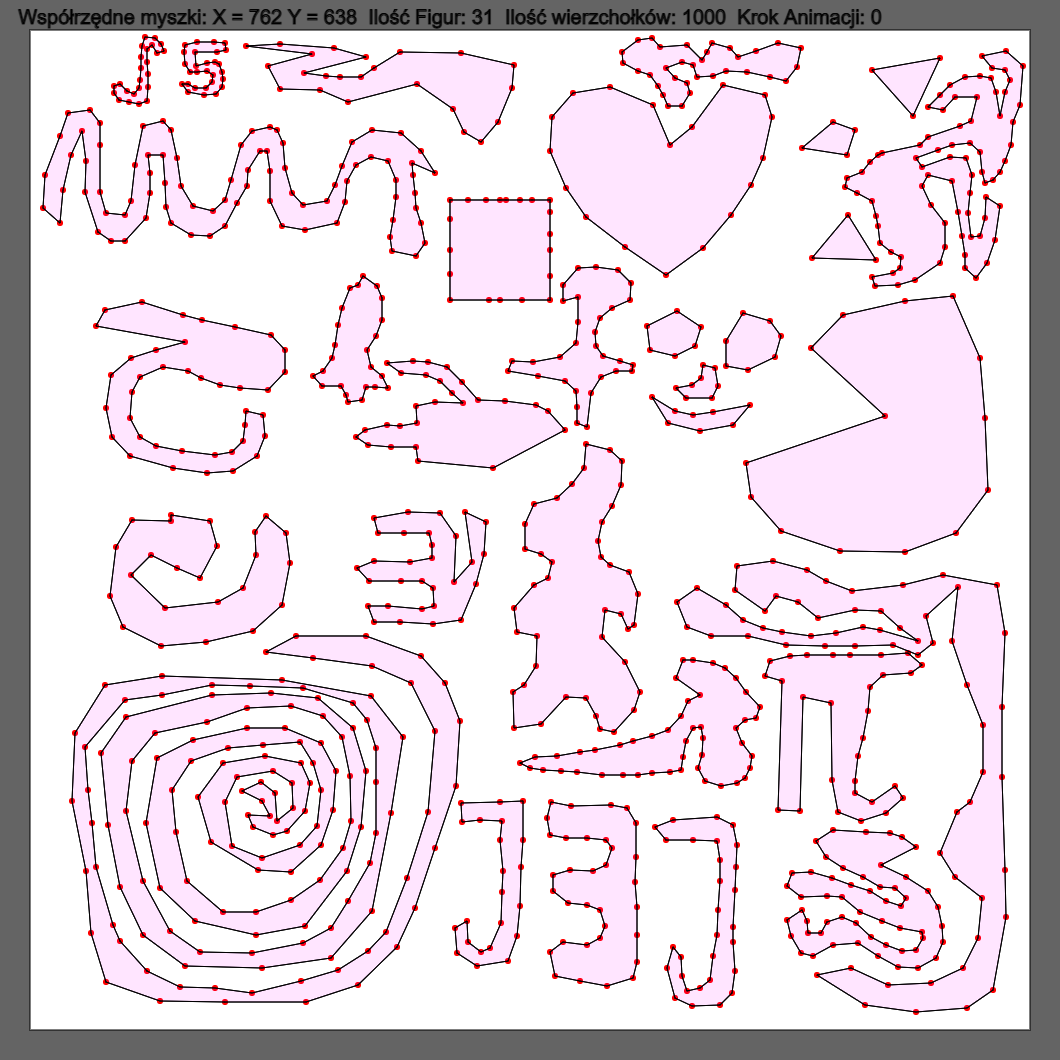
\includegraphics[width=.45\textwidth]{rys11.png}\hfill
    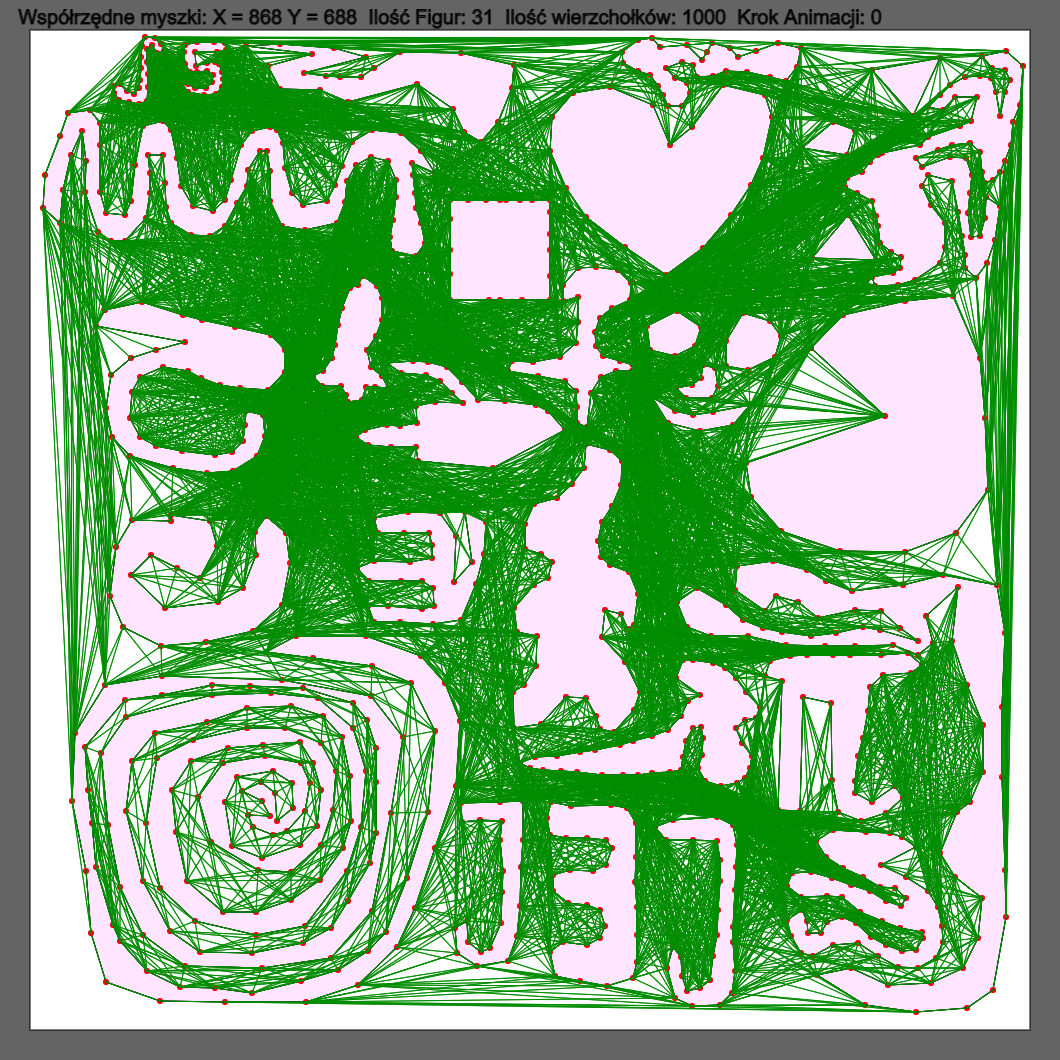
\includegraphics[width=.45\textwidth]{rys12.png}
\end{figure}
\newpage

\subsection{Symetryczne dane}
\qquad 

\begin{figure}[h]
\centering
\caption \centering{Przykładowy symetryczny zestaw danych i jego graf widoczności}
    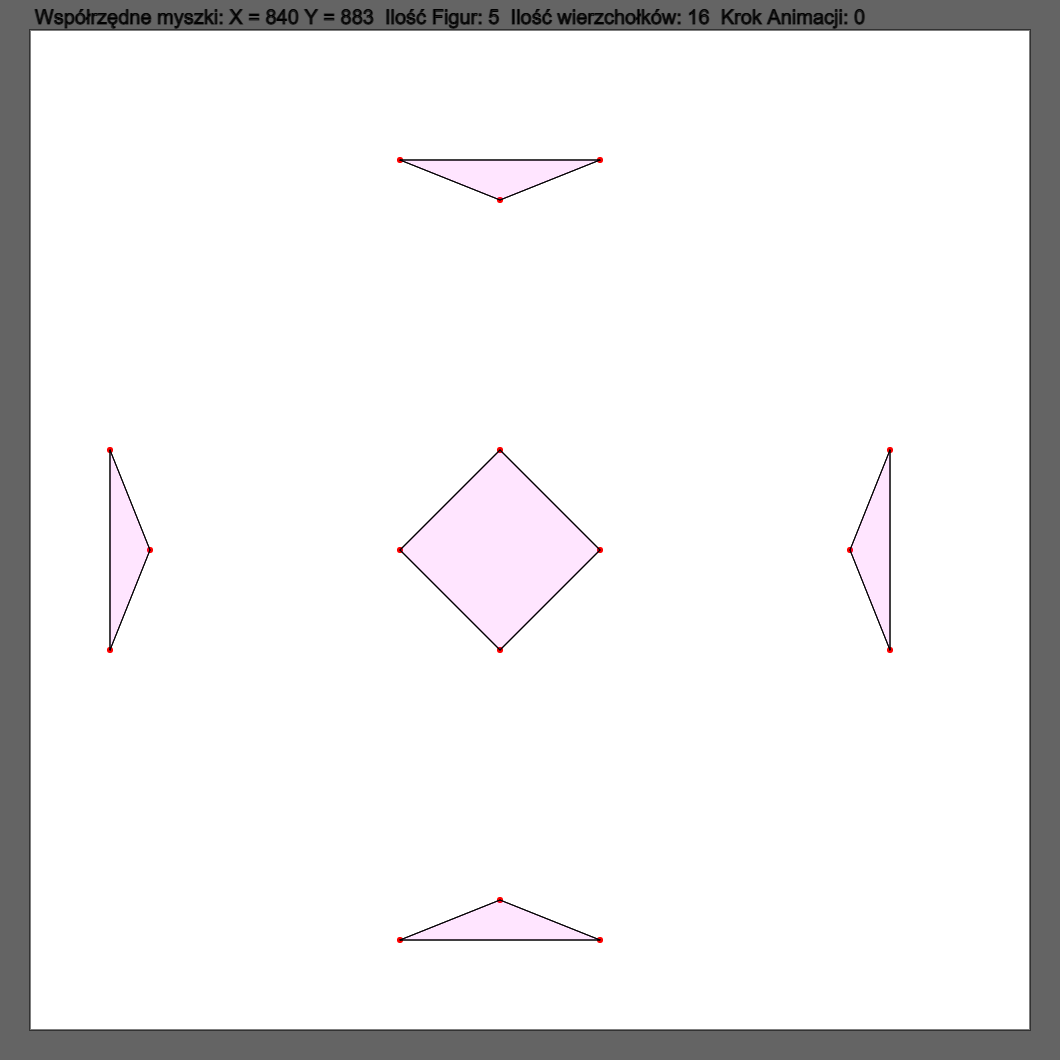
\includegraphics[width=.45\textwidth]{rys13.png}\hfill
    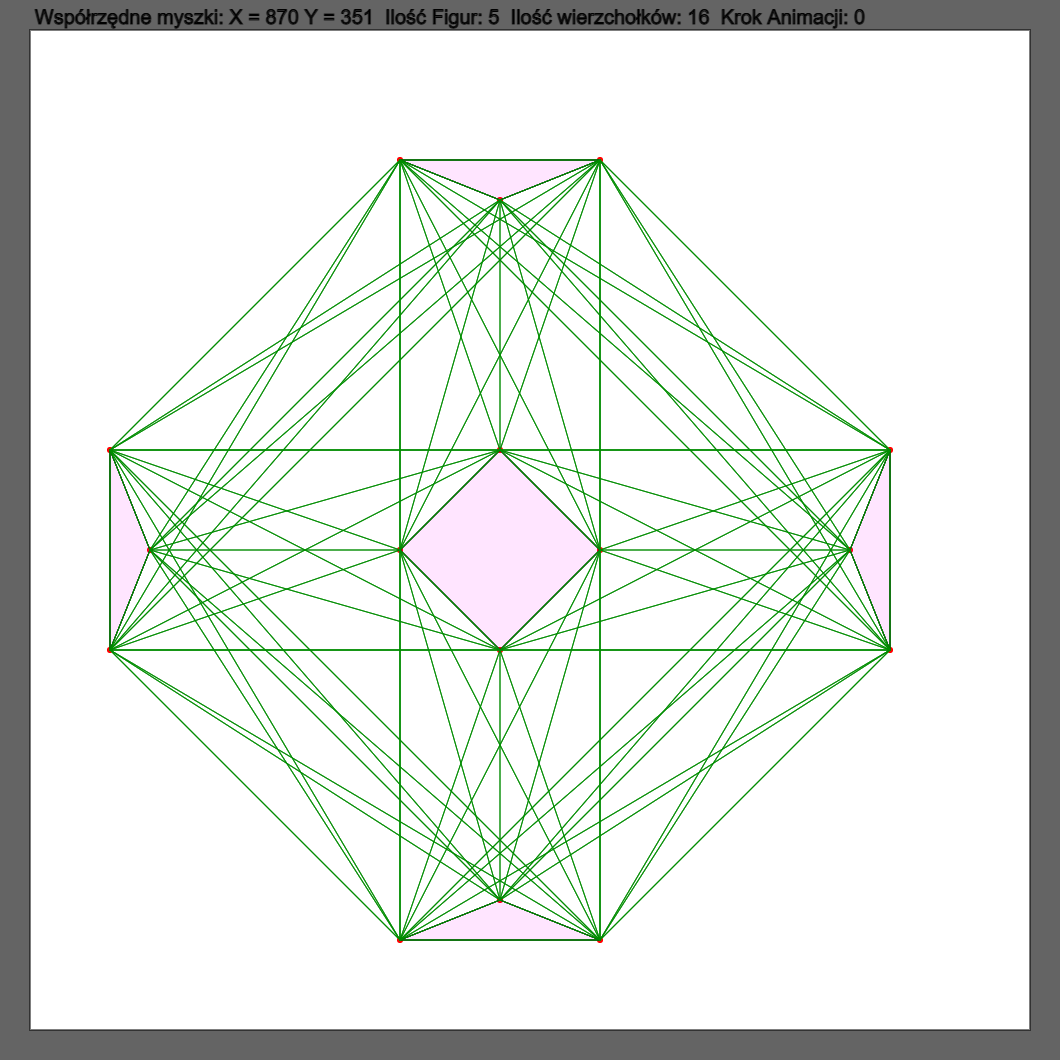
\includegraphics[width=.45\textwidth]{rys14.png}
\end{figure}


\section{Podsumowanie}
\qquad Zaimplementowany algorytm pozwala określić graf widoczności dla zadanych danych wejściowych. Dodatkowo osiąga on zauważalnie lepsze wyniki czasowe w porównaniu do algorytmu naiwnego, co świadczy o jego poprawnej implementacji.  Aplikacja stworzona na potrzeby wizualizacji grafu pozwala wyświetlenie odpowiednich animacji, dzięki którym możliwe jest poznanie algorytmu wyznaczającego graf widoczności. Implementacja algorytmu wymagała użycia wielu technik związanych z algorytmami geometrycznymi poznanych na wcześniejszych laboratoriach. Poza koncepcją algorytmów zamiatania do takich metod zalicza się sortowanie punktów na podstawie ich kąta, użycie wyznacznika do określania wzajemnego położenia punktów, oraz - co mniej oczywiste - określanie kierunku w jakim został zadany wielokąt na podstawie fragmentu jego otoczki wypukłej.


\begin{thebibliography}{9}
\bibitem{texbook}
de Berg M., Van Kreveld M., Overmars M. \emph{Geometria obliczeniowa. Algorytmy i zastosowania}
\end{thebibliography}

\end{document}